\setcounter{chapter}{7}
\chapter{固体物理概述}\label{chap:Solid-state_introduct}
\section{固体的分类与结合}

\subsection{固体的分类:~晶体、非晶体与准晶}
固体是由大量原子(或离子)组成的复杂体系。根据内部的原子、离子的排布规范情况,固体一般可分为晶体(包括单晶与多晶)、非晶体和准晶。晶体与非晶体的最本质差别在于组成晶体的粒子(原子、离子或分子等)是长程有序排列的,而非晶体中,除了最近邻的粒子有可能有序排列外,一般粒子都呈现无规则堆积。石英的两种结构(石英晶体和石英玻璃)很好地说明了这两个不同序的区别,如图\ref{Fig:SSI-01} 所示。
\begin{figure}[h!]
\centering
\vspace*{-0.18in}
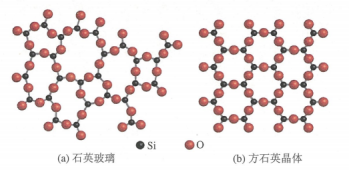
\includegraphics[height=1.85in,width=3.8in,viewport=0 0 84 40,clip]{Figures/2D-SiO2.png}
\caption{\small \textrm{Two structure of $\mathrm{SiO}_2$.}}%(与文献\cite{EPJB33-47_2003}图1对比)
\label{Fig:SSI-01}
\end{figure}
在两种结构一个Si原子周围都有三个O原子,这表示短程有序(化学组分比相同)。石英晶体还呈现一个由六边形组成的规则网格的二维结构 ,这就是长程有序,石英玻璃则没有这一额外的规则性。因此,{\heiti 晶体是指其内部的原子、离子或分子在空间按一定的周期性排列(即晶体的周期性结构)、长短程均有序的固体物质,长程序使得晶体具备平移不变性。}

许多重要的固体材料都是晶体,如大多数固态的金属与合金等。非晶体如橡胶 、塑料 、玻璃和松脂等,其原子排列没有周期性 ,不存在长程序,但保留有原子排列的短程序。固体的长程序导致晶体具有一些共同的特征,如规则外形、均匀性、各向异性、解理性、具有特定的熔点、宏观和微观对称性等。例如晶体具有固定熔点是由于当加热到一定温度(熔点)时,晶体内的结合键将同时断裂,破坏其规则排列的状态。而非晶体由于缺乏长程序,结合键能是变化的。当加热非晶体时,弱的键会在更低的温度断裂,因此非晶体宏观表现为慢慢熔化 ,没有固定的熔点。根据原子排列有序度的尺寸大小,晶体又可分为单晶与多晶。单晶在整体范围内原子都是规则排列的,因此其具有规则外形 ,一般呈现为平滑的凸多面体。受外力时,晶体可沿某些晶面劈裂开(晶体的解理性),这些晶面称为解理面。%晶体呈现出的光滑凸多面体往往是一些解理面。
多晶体则由许多细微晶体颗粒组成,在各晶粒范围内,原子是有序排列的,而晶粒间的取向是不同的(如图\ref{Fig:SSI-02}所示),如金属以及陶瓷材料等。不论单晶还是多晶 ,在微米量级范围内,微观粒子排列都具有长程和短程有序。晶体这种整体有规则排列结构使得数学处理相对简单 ,理想的晶体结构是固体物理领域理论的出发点。
\begin{figure}[h!]
\centering
\vspace*{-0.18in}
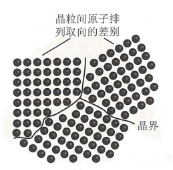
\includegraphics[height=1.85in,width=2.0in,viewport=0 0 45 40,clip]{Figures/Polycrystal.png}
\caption{\small \textrm{Schematic diagram of Polycrystalline. }}%(与文献\cite{EPJB33-47_2003}图1对比)
\label{Fig:SSI-02}
\end{figure}

非晶体与液体类似,具有短程有序而长程无序的结构特征,非晶体又称玻璃态,可看成是黏滞性很大的过冷液体。晶体的长程有序结构使其内能处在最低状态,而非晶体因为长程无序,内能没有处于最低状态,所以固体非晶态本质上是一种亚稳相。与此对应的是一类新型的固体材料——非晶态材料,包括我们日常所见的各种玻璃、塑料、高分子聚合物以及新近发展起来的金属玻璃、非晶态合金、非晶态半导体及非晶态超导体等。由于结构不同,非晶态材料具有许多晶体所不具备的优良性质,如优异的机械特性(强度高、弹性好)、电磁学特性 、化学特性(稳定性高、耐蚀性好、抗辐射等)、电化学特性及优异的催化活性等,已成为一类发展潜力很大的新材料,由于其用途广泛,备受青睐。不过由于非晶体的结构比晶体要复杂得多,无法直接将描述和研究晶体的理论直接应用到非晶体的研究中 ,因此必须寻找新的方法。经过几十年的努力,非晶态物理学的研究虽然取得了很大进展,但与基本成熟的晶态物理学相比,还处在发轫阶段,有大量的课题需要进一步研究。

还有一类固体物质,由于其结构的有序程度介于晶体和非晶体之间,因此被称为准晶体。具体而言,准晶具有与晶体相似的长程有序原子排列,但却不具备晶体所应有的平移对称性。因而准晶可以具有晶体所不允许的宏观对称性(如五重对称轴)。%
1982年美国国家标准局D. Shechtman等人在用快速冷却方法制备Al-Mn合金时发现了具有五重旋转对称但并无平移周期性的合金像(如图\ref{Fig:SSI-03}),彻底地改变了上述晶体局限定理的传统观念。
\begin{figure}[h!]
\centering
\vspace*{-0.1in}
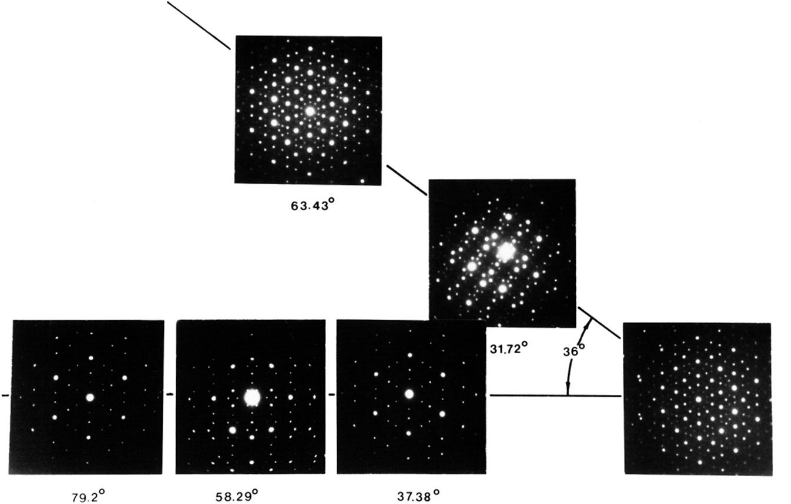
\includegraphics[height=1.85in,width=3.0in,viewport=0 0 791 504,clip]{Figures/quasicrystal.png}
\caption{\small \textrm{Selected-area electron diffraction patterns taken from a single grain of the Al-Mn icosahedral phase. Cited from \inlinecite{PRL53-1951_1984}. }}%(与文献\cite{EPJB33-47_2003}图1对比)
\label{Fig:SSI-03}
\end{figure}
根据晶体局限定理,普通晶体内只能允许二次、三次、四次或六次旋转对称轴存在,准晶是原子的排列存在五次和六次以上对称轴的一种特殊晶体。究其原因,因为传统的晶体局限定义存在缺陷,它把原子排列有序和三维周期性混为一谈:~即从一个更自然的角度,非晶与晶体的区分在于其内部结构中的原子、离子或分子是否呈有序排列,而有序是否会导致三维周期性在没有被证实的情况下,被默认为常识接受了。国际晶体学联合会下设的非周期晶体学术委员会在1992年建议,将晶体的定义改为``能够给出明锐衍射的固体''。在Shechtman发现准晶体后,实验室中还发现了许多稳定和亚稳准晶,这些通常是含铝的金属合金。2009年,在俄罗斯东部获取的一块铝铜铁矿($\mathrm{Al}_{63}\mathrm{Cu}_{24}\mathrm{Fe}_{13}$)上发现了天然准晶体。实际上 ,数学家在准晶体发现之前已经从理论上预言了准晶体的存在。1976年Roger Penrose构造了一种由两种拼图拼接而成的具有五次对称性的图案。
\begin{figure}[h!]
\centering
\vspace*{-0.1in}
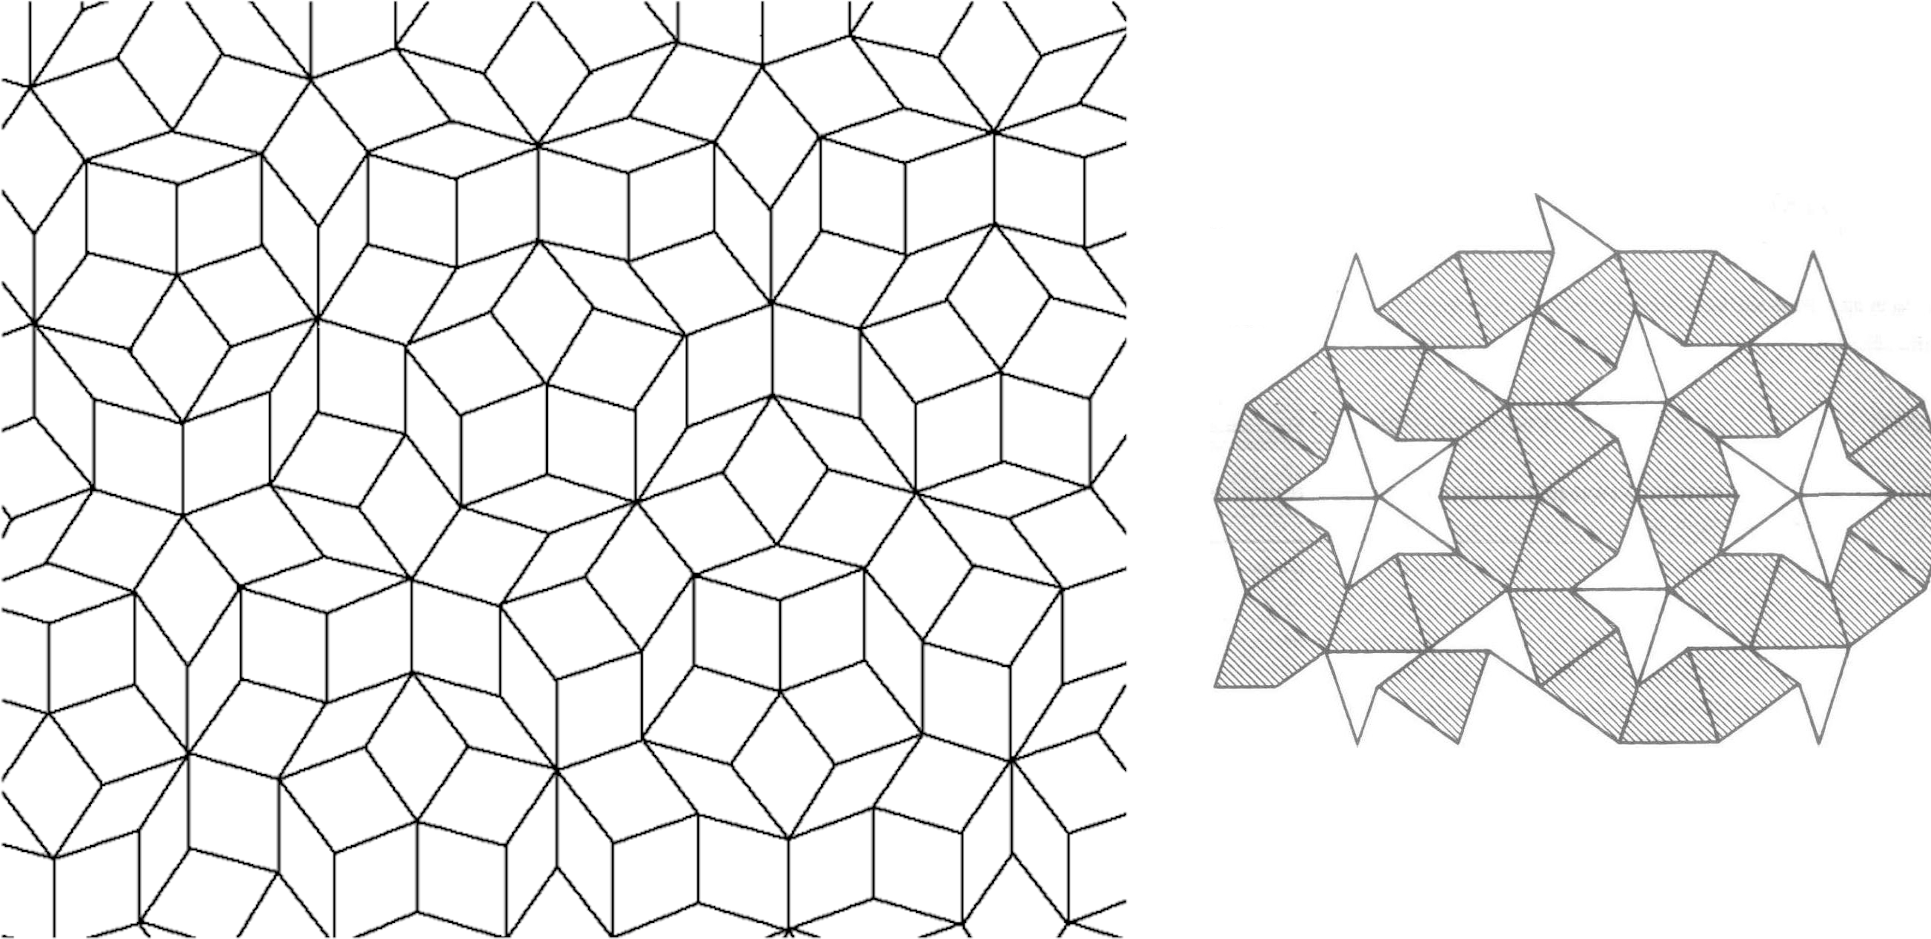
\includegraphics[height=1.85in,width=3.7in,viewport=0 0 1931 939,clip]{Figures/Penrose-puzzle.png}
\caption{\small \textrm{A schematic diagram of 2D-Penrose tiling.}}%(与文献\cite{EPJB33-47_2003}图1对比)
\label{Fig:Penrose-puzzle}
\end{figure}
图\ref{Fig:Penrose-puzzle}为二维空间的Penrose拼图(左)及其五重对称性示意(右),由内角为$36^{\circ}$、$144^{\circ}$和 $72^{\circ}$、$108^{\circ}$的两种菱形组成 ,能够无缝隙无交叠地排满二维平面。这种拼图没有平移对称性 ,但是一种长程有序的结构,并且具有晶体所不允许的五次旋转对称性。准晶体的这种特殊结构对其物理性能有明显的影响,使其具有独特的属性 ,如高电阻 、低热导率、低摩擦系数、良好的耐磨性和抗氧化性 、高硬度 、高温塑性等优异性能等 ,已被开发为有用的材料,如表面防护涂层、隔热材料 、储氢材料、太阳能工业薄膜材料等准晶复合材料。准晶体的实验发现被认为是固体物理学近几十年来的一项重大突破,它一方面极大地深化了我们对晶体学 、衍射物理和凝聚态物理的认识 ,另一方面 ,准晶体的各种独特性质使准晶体具有潜在的应用价值。因此D. Shechtman一人独享了2011年诺贝尔化学奖。但是除了一维情况外 ,目前无论是实验还是理论方面准晶体的物性研究都还处于起始阶段。

\subsection{晶体结合:~离子晶体、共价晶体、金属晶体、分子晶体}
晶体中原子、离子或分子由于粒子间相互作用而结合成一定的稳定结构,晶体的总能量要比自由状态的原子或分子的总能量低。晶体的结合能定义为自由原子能与晶体能量之差。不同晶体的结合能相差很大 ,从0.01eV到10eV不等,结合能决定了晶体的性质,主要与晶体中原子间的互作用(包括吸引作用和排斥作用)相关。图\ref{Fig:SSI-04}示意的是双原子体系间互作用的典型势能曲线,近似的数学表达式为
\begin{figure}[h!]
\centering
\vspace*{-0.1in}
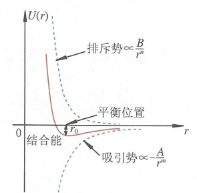
\includegraphics[height=1.85in,width=2.5in,viewport=0 0 50 40,clip]{Figures/Interaction-2_Atoms.png}
\caption{\small \textrm{原子间相互作用.}}%(与文献\cite{EPJB33-47_2003}图1对比)
\label{Fig:SSI-04}
\end{figure}
\begin{equation}
	U(r)=-\dfrac{A}{r^m}+\dfrac{B}{r^n}
	\label{eq:SSI-01}
\end{equation}
式中r表示两原子间距。参数A、B、n、m>0且m<n,是与晶体性质相关的常数,负号表示吸引势,正号表示排斥势,斥力高度短程,而引力是长程的。两原子间的互作用力由势函数的梯度决定:
\begin{equation}
	f(r)=-\dfrac{\mathrm{d}U(r)}{\mathrm{d}r}
	\label{eq:SSI-02}
\end{equation}
当两原子间距$r\rightarrow\infty$,势能为零,作用力为零,表示自由原子状态的能量。当两原子逐渐靠拢且$r\rightarrow r_0$时,势能为负,随着原子间距r减小而逐渐减小,此时$f(r)<0$,表明引力大于斥力。到达平衡位置$r=r_0$时,势能取最小值$f(r)=0$,则,表明引力与斥力达到平衡。当两原子间距继续减小,即$r<r_0$,随着原子间距r减小,势能迅速增加,此时$f(r)>0$,表明斥力大于引力。

晶体的结构和性质与晶体中原子结合作用的性质密切相关。固体中粒子的相互吸引完全根源于电子的负电荷与原子核的正电荷之间的静电吸引相互作用,是晶体中原子或分子不同结合键的反映,一般具有多种表现形式。在根据晶体中最小重复单元的原子间相互作用类型 ,可将晶体分为几种典型类型:离子晶体、共价晶体、金属晶体和分子晶体,前三种为强键结合 ,后一种为弱键结合。图\ref{Fig:SSI-05}是这几种典型类型的示意图。尽管在不同晶体中引力(键)的形式差别很大,然而在所有固体中排斥力的来源几乎是相似的,主要来自于同种电荷的库仑排斥力(如核排斥力)和泡利不相容原理所导致的量子效应。在吸引力作用下原子聚合,就会出现电子云重叠现象,由泡利不相容原理可知 ,要求部分电子被激发到没有被占据的更高能量 态上,因而使得系统的总能量增加 ,可看成是对斥力的贡献。
\begin{figure}[h!]
\centering
\vspace*{-0.1in}
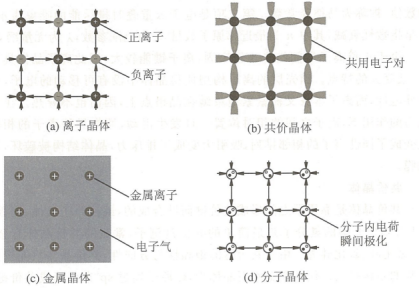
\includegraphics[height=1.85in,width=2.5in,viewport=0 0 90 70,clip]{Figures/Four_Crystal-type.png}
\caption{\small \textrm{晶体的结合类型示意.}}%(与文献\cite{EPJB33-47_2003}图1对比)
\label{Fig:SSI-05}
\end{figure}

\subsubsection{离子晶体} 
离子晶体是由正负离子交替排列而成的,每个离子周围最近邻的都是异性电荷离子,离子间库仑作用的净效果表现为吸引性,因此其结合力主要来自于正、负离子间的Coulomb吸引作用,习惯上称为离子键。离子键是易于失去电子形成阳离子的原子和易于俘获电子形成阴离子的原子间形成的强极性相互作用。
典型的离子晶体有碱金属元素和卤族元素的结合物,如NaCl和KCl。Na原子的电离能为5.14~eV,Cl原子的电子亲和能\footnote{电子亲和能是指中性原子获得一个电子形成负离子时所释放的能量。}为3.62~eV,故从自由的Na和C1原子形成$\mathrm{Na}^+$和$\mathrm{Cl}^-$所需能量为$5.14-3.62=1.52\mathrm{eV}$,实验结果显示,%离子间静电相互作用,Na+和Cl-间距离的变化由图5.1.3中红线所示,NaCl中的结合能为-4.2eV,$\mathrm{Na}^+$和$\mathrm{Cl}^-$的距离为0.24nm。
在NaCl晶体中%情况有所不同,
离子的平衡位置间距离为0.28nm,晶体中每对离子的结合能为7.84eV, 因此NaCl晶体中$\mathrm{Na}^+$和$\mathrm{Cl}^-$的结合能为$7.84-1.52=6.32\mathrm{eV}$,%结合成离子晶体后总能量比分离原子的总能量低。
在离子晶体中,不同原子通过获得或失去电子形成闭壳层的离子,电荷近似球对称,故当离子间距较远时可把离子当点电荷处理,同时也说明了离子键是无方向性的,每个离子周围吸引尽可能多的异性电荷离子,原子排列结构部分取决于正负离子的相对大小。对于一个有N个原胞的晶体,总的势能可以写成
\begin{equation}
	U=N\bigg[-\dfrac{\alpha q^2}{4\pi\varepsilon_0r}+n\lambda\exp\big(-\dfrac r{\rho}\big)\bigg]
	\label{eq:SSI-03}
\end{equation} 
上式中第一项是正负离子交替的Coulomb能,其中$\alpha$是一个完全取决于晶体结构的无量纲的数值,称为Madlung常数。第二项是电子云重叠时排斥能的唯象表示,排斥势呈指数性衰减,其中$n$为最近邻原子数目,$\rho$为范围参数,$\lambda$为无量纲参数。

由于正、负离子之间结合比较牢固,离子键能较大,因此离子晶体具有熔点高、硬度大的特点。满壳层的离子构型使得晶体中没有可自由移动的电子,因而不具备导电条件,而离子本身又被紧紧地束缚在晶格点上,因而也不导热。在外部机械力的作用下,离子之间的相对位置一旦发生滑动,原来异性离子的相间排列就变成了同性离子的相邻排列,吸引力变成了排斥力,晶体结构被破坏,因而质地脆。

\subsubsection{共价晶体} 
共价晶体是靠原子之间形成共价键而结合成的,亦称原子晶体、同极晶体。常见的共价晶体有金刚石、硅、SiC、$\mathrm{SiO}_2$等。由于共价键的饱和性与方向性,共价晶体只能按照某种特殊的结构排列。例如在金刚石晶体中,C原子通过$sp^3$杂化形成共价键,由于共价键的方向性,每个原子与相邻的原子都是以四面体方式结合,导致这种结的排列方式空间占用率很低。

由于共价键比离子键具有更高的结合能 ,非常稳定,因此共价晶体具有高力学强度、高熔点、高沸点和低挥发等特性。所有的价电子都参与成键,不能自由运动 ,因而低温时电导率很低,温度增加或加入杂质时电导率增大 ,如半导体Si、Ge等。

\subsubsection{金属晶体} 
金属晶体基本特点每个原子的价电子不再束缚在某一特定的原子上,而是遍及在整个晶体内。金属元素的阳离子可看成是浸没在近均匀的电子海洋中 ,正离子与电子之间的Coulomb力提供了聚合作用,而且体积越小时,Coulomb能越低,聚合作用越强烈。但是当体积缩小,由Thomas-Fermi统计知道,动能正比于电子云密度的三分之二次方,即会增大电子的动能 ,这是排斥势的来源之一;排斥势的另一来源是Pauli不相容原理 ,当原子实靠近时电子云重叠产生强烈的排斥作用。

金属原子结合比离子键和共价键结合都弱,但仍属于强结合。例如金属Na的熔点大约是$400^{\circ}\mathrm{C}$,NaCl的熔点大约是$1100^{\circ}\mathrm{C}$,金刚石的熔点大约是$4000^{\circ}\mathrm{C}$。金属键是无方向性也无饱和性的,故金属元素总是倾向于密堆积的结构:~面心立方或六角密排列,而不倾向于排列疏松的结构,如金刚石结构。金属所具有的特性,如金属光泽(即对可见光强烈反射)、良好的导电、导热性,富有延展性和可塑性等,都与这些在整个金属内可自由运动的非局域化电子有关。例如对于金属在形变过程中不易断裂的典型特征,可以进行以下简单的定性解释:~周期排列的正离子之间有可流动的电子,使得金属键在整个晶体范围内起作用,因而断开它比较困难;另外,受外力作用金属原子的移位滑动不影响离域的电子对金属离子的维系作用,因而对原子移动时克服势垒起到调节作用。也正是由于价电子被所有原子所分享,因此如果原子大小相近,可或多或少按任意比例形成不同的合金。

过渡金属(如Fe、Ni、Ti、Co 等)的结合机制更为复杂,这是因为除了$s$电子行为像自由电子外 ,还有较局域化的$3d$电子和邻近的电子形成共价键,有时这些$d$电子和$s$电子强烈杂化形成更复杂的结合。

\subsubsection{分子晶体} 
分子晶体是具有饱和结构的原子或分子依靠van der Waals力相结合而成的。不像前述的三种结合中原子价电子状态在形成晶体后都发生了改变,形成分子晶体的原子或分子电子状态没有改变。van der Waals力有三种不同类型:极性分子之间的分子固有偶极矩之间的力,为Keeson力;极性分子与非极性分子的感应偶极矩之间产生的力,为Debye力;中性分子之间主要是瞬时电偶极矩之间的感应作用力 ,为London力或色散力,这是所有分子都具有的互作用力。

以中性分子的分子晶体(如惰性气体元素、双原子分子$\mathrm{H}_2$、$\mathrm{O}_2$、$\mathrm{N}_2$等)为例,van der Waals结合是一种瞬时的电偶极矩感应作用,排斥势则是由于Pauli不相容原理导致的,两原子或分子间的总势能可以表示为Lennard-Jones势:
\begin{equation}
	U=4\varepsilon\bigg[\big(\dfrac{\sigma}r\big)^{12}-\big(\dfrac{\sigma}r\big)^6\bigg]
	\label{eq:SSI-04}
\end{equation}
式中$r$为原子间距,$\varepsilon$和$\sigma$是经验参数,可由实验测得。其中$r^{12}$项由实验数据拟合给出,$r^6$项可通过简单的物理模型推导给出。分子1、2 相距$r$,第一个分子瞬时偶极矩为$p_1$,其在第二个分子处的电场正比于$E\propto p_1/r^3$,分子2将被诱导产生偶极矩$p_2\propto E$,从而两个分子间偶极矩作用能为$\dfrac{p_1p_2}{r^3}\propto\dfrac{p_1^2}{r^6}$。因此分子间的van der Waals力正比于$1/r^7$,随着距离增加,van der Waals力将迅速减小。

van der Waals力是非常弱的吸引力,因而分子晶体一般有非常低的熔点和沸点,而且参与分子间相互作用的电子是局域的,故分子晶体通常也不导电。如固态氨的结合能仅仅0.8eV/原子,熔点-$189^{\circ}\mathrm{C}$,固态氢的结合能仅仅0.01eV/原子,熔点-$259^{\circ}\mathrm{C}$,固态甲烷的结合能仅仅0.1 eV/原子,熔点-$183^{\circ}\mathrm{C}$。

\begin{figure}[h!]
\centering
\vspace*{-0.1in}
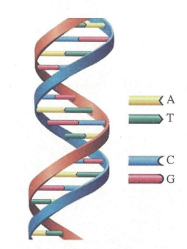
\includegraphics[height=1.85in,width=1.5in,viewport=0 0 70 90,clip]{Figures/Double_helix-structure-DNA.png}
\caption{\small \textrm{DNA的双螺旋结构.}}%(与文献\cite{EPJB33-47_2003}图1对比)
\label{Fig:DNA}
\end{figure}
当分子包含H原子时形成一类特别强的van der Waals力,称为H键。由于H原子仅仅包含一个电子,当与一个电负性强的元素结合时,电子倾向于聚集在电负性强的元素附近,导致带正电的裸露H原子核(就是一个质子)处在分子边缘,故还可以与另一极性分子的负电荷端发生相互作用。裸露的H原子核比一般的原子的半径小很多,因此与另一极性分子的负电荷部分能靠得很近,形成较强的van der Waals力。普通纸中纤维间的主要结合力来自纤维素纤维间的H键作用,遇水时H键解体,这就是为什么普通纸在完全被水湿透之后,就几乎完全失去了强度。H键也广泛存在于生物体中,是一种理解细胞活动的重要机制。例如脱氧核糖核酸(DNA)的双螺旋结构(图\ref{Fig:DNA}),主要是两条互补的多聚脱糖核苷链由H键的作用配对在一起而形成的,DNA的复制机制正是依赖于这种结构。在细胞中分子的平均动能大约为0.04eV, 和H键大小同一量级。这就意味着通过分子的碰撞,氢键很容易断裂。因此H键不是非常牢固的,它们仅仅是简单地连接,也正因为如此,在细胞中H键起着重要的作用。另一方面,在DNA链内部的强键将原子紧紧结合在一起,不能仅仅通过分子碰撞而断裂。2013年11月,中国科学家利用原子力显微镜在国际上首次发布了H键的照片(图\ref{Fig:H-bond}),实现了H键的实空间成像,为``氢键的本质''这一化学界争论了80 多年的问题提供了直观证据。
\begin{figure}[h!]
\centering
\vspace*{-0.1in}
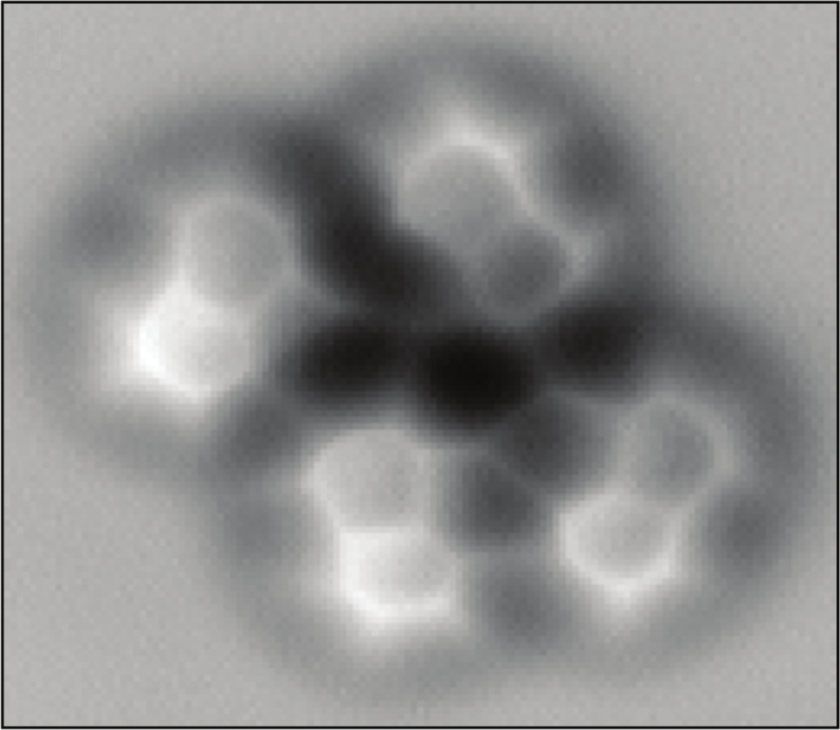
\includegraphics[height=2.15in,width=2.5in,viewport=0 0 840 730,clip]{Figures/Image-of-H_bond.png}
\caption{\small \textrm{中国科学院国家纳米科学中心发布的H键的照片.}}%(与文献\cite{EPJB33-47_2003}图1对比)
\label{Fig:H-bond}
\end{figure}

\begin{table}
  \centering
  \caption{晶体类型}
  \begin{tabular}{c|@{\extracolsep{\fill}}m{2.7cm}<\centering|m{2.7cm}<\centering|@{\extracolsep{\fill}}m{2.7cm}<\centering|@{\extracolsep{\fill}}m{2.7cm}<\centering}
    \toprule
    晶体类型 & 离子晶体 & 共价晶体 & 分子晶体 & 金属晶体 \\
    \midrule
    组成粒子 & 正、负离子 & 原子 & 分子 &金属离子和自由电子 \\
%    & & & & 自由电子\\
    \hline
    键 & 离子键 & 共价键 & van der Waals力 & 金属键 \\\hline
    结合能 & 4$\sim$14eV &2$\sim$10eV &0.02$\sim$0.3eV &0.7$\sim$6 eV \\\hline
    性质   & 熔点高、硬度大。多数易溶于水等极性液体,低温下一般不导电、不导热(溶于水或熔化时可导电)  & 熔点极高、硬度大,不导电,延展性很差,不能在一般溶剂中溶解 & 熔点、沸点低,硬度低,固态不导电 & 具有金属光泽,易导电、导热,有较好的延展性和可塑性   \\\hline
    实例   & NaCl ($E=3.28\mathrm{eV/atom}$) & 金刚石 ($E=3.28\mathrm{eV/atom}$) & $\mathrm{CH}_4$ ($E=3.28\mathrm{eV/atom}$) & 金属Na ($E=1.1\mathrm{eV/atom}$)\\
    \bottomrule
  \end{tabular}
  \label{Tab:SSI-01}
\end{table}

为了研究方便,我们将晶体划分为上述几种典型类型,表\ref{Tab:SSI-01}总结了这几种典型类型的基本特点。实际上,不同类型的晶体并不存在绝对的界限,更可能是具有几种结合形式的复杂结合。例如,离子键和共价键是两种极端的情形,在离子键中电子从一个原子完全转移到另一个原子中 ,而共价键中电子完全被两个原子分享。实际的原子之间化学键往往是介于这两种极端情形之间,对于一个给定的键,我们可以从多大程度上具有离子性或共价性结合给予适当的描述,通常引入电离度的概念来描述共价结合中的离子成分。除了原子之间的化学键,晶体的形成也可能有分子键的参与。石墨是一个典型的例子(图\ref{Fig:Graphe}),由具有六角蜂房结构的二维石墨烯层堆积而成,层内的C原子通过$sp^2$杂化形成强的共价键结合,C原子的最外层还留下一个能够在层内自由移动的价电子 ,这解释了为什么石墨具有接近金属的光泽和在某一方向的导电性。层与层之间靠弱的van der Waals力结合,因此不同层能相对容易地彼此滑动 ,这就是石墨能作为润滑剂和铅笔的缘故。

\begin{figure}[h!]
\centering
\vspace*{-0.1in}
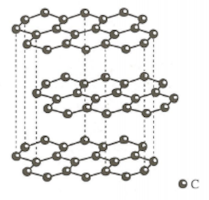
\includegraphics[height=1.75in,width=1.6in,viewport=0 0 55 50,clip]{Figures/Graphe.png}
\caption{\small \textrm{石墨的晶体结构.}}%(与文献\cite{EPJB33-47_2003}图1对比)
\label{Fig:Graphe}
\end{figure}

\section{晶体结构学基础}
结构是认识和研究物质的基础,从根源上揭示了固体的一系列现象和性质。晶体最本质的结构特性是晶体中原子的周期性排列,或称为晶体的平移对称性,它的存在大大简化了所需处理的问题。%这一节我们将介绍
本部分将介绍如何描述晶体的周期性结构、对称性以及晶体结构的测定等晶体结构学的一些基础知识。

\subsection{晶格与平移对称性}
晶体结构学关心的是晶体的几何周期性结构,为了形象地描述晶体结构,将晶体中原子、离子或分子的重复单元数学抽象为几何学上的点,所有点的集合所连成的空间周期性排列网格定义为晶格,也称Bravais格子。选择任意一点作为原点,Bravais格子中所有点都可由平移矢量表示为
\begin{equation}
	\vec R_n=n_1\vec a_1+n_2\vec a_2+n_3\vec a_3\qquad (n_1,n_2,n_3\mbox{均为整数})
	\label{eq:SSI-06}
\end{equation}
其中$\vec a_1$、$\vec a_2$、$\vec a_3$是不共面的基矢,称为Bravais格子的基矢,$\vec R_n$称为Bravais格子的格矢,端点称为格点。沿任意一格矢平移,布拉菲格子不变。注意基矢$\vec a_1$、$\vec a_2$、$\vec a_3$的选择并不唯一,例如$\vec a_1+\vec a_2$、$\vec a_2$、$\vec a_3$也能产生与式\eqref{eq:SSI-06}相同的Bravais格子。图\ref{Fig:SSI-07}示意了二维格子中基矢的几种不同取法。由定义可看出布拉菲格子是一个无限延展的点阵,点阵上所有格点完全等价(几何位置上等价、周围环境都相同),它代表了晶体最本质的特性一 平移对称性。然而,固体是一个物理的结构,不是一套数学点的集合。对于一个实际的晶体结构,必须考虑每个布拉菲格点上所代表的具体物理内容,这就是基元,它可能是单个原子或离子,也可能是由多个原子或离子组成的原子(或离子)团。因此晶体结构可以概括描述为基元以相同的方式重复放置在点阵格点上所构成,即

晶体结构 = 布拉菲格子(数学抽象)+ 基元(物理内容)

晶体结构的描述不仅需要知道布拉菲格子的基矢、、,还需要知道基元所包含的具体内容。根据基元所包含的内容,布拉菲格子有简单格子与复式格子之分。基元中仅包含一个原子的晶格称为简单格子,原子所构成的列阵与此晶体的布拉菲格子完全相同,选取合适的原点,布拉菲格点即可表示原子的平衡位置。基元中包含两个或两个以上原子的晶格称为复式格子,此时还需要引入一组合适的矢量、、…、心描述个不同原子在基元中的相对位置,则每个不等价原子的平衡位置可由平移矢量决定。由此可见 ,基元中每个不同原子所构成的阵列都与此晶体的布拉菲格子相同。这些由基元中不同原子的平移矢量所构成的阵列常称为子格子,整个复式格子可视为 v 个与晶体的布拉菲格子相同的子格子套构而成。因此 ,晶体结构的几何描述由布拉菲格子的基矢、、和形成基元原子的位置矢量、、…、共同决定。图 6.2.2示意了基元由两个不同原子组成的二维石墨烯复式晶格,属于三角(或六角)二维布拉菲格子,其中原子A、B 表示基元中两个不同原子。



严格地说 ,完全理想的无限延伸的完美晶体是不存在的,在实际晶体材料中,必然存在以下几种不完美性破坏其周期性结构:

(1)实际晶体具有一定的尺寸大小,存在表面和边缘 ,不是无限延伸的。

(2)当温度 T > 0 K 时,原子在它们的平衡位置附近热振动导致晶格的畸变等。

(3)实际晶体总是包含一些缺陷和杂质。



图6.2.2 基元由两个不同原子组成的二维石墨烯复式晶格


\subsection{基本重复单元 :原胞和晶胞}

原胞,又称固体物理学原胞,初基原胞,是将整个晶格划分为只包含一个布拉菲格点的周期性重复单元。通过重复堆积原胞将精确地填满整个空间,没有重叠也没有遗漏。原胞常取以基矢为棱边的平行六面体(图 6. 2. 3),体积为



上述取法只是习惯的取法,原则上原胞可以有任意多种取法,只要满足晶体的最小重复单元这个条件。无论如何选取,原胞均有相同的体积,每个原胞含有一个格点。另一种重要的取法是维格纳-塞茨(Wigner-Seitz)原胞,即以某个格点为中心,做其与邻近格点的中垂面,这些中垂面所包含最小体积的区域。这种取法不仅反映了晶体的平移对称性,并且反映了与相应的布拉菲格子完全相同的对称性,是一种对称性原胞,不依赖于基矢的选择。在二维晶格中则是以某个格点为中心,做其与邻近格点的中垂线,这些中垂线包含最小面积的区域,即维格纳 -塞茨原胞。



有时,为了更加直观地反映出晶体的宏观对称性,取一个包含若干个原胞的平行六面体作为重复单元,该重复单元被称为结晶学原胞,简称晶胞或单胞,它是保持晶体宏观对称性的基本结构。晶胞一般为布拉菲格子中对称性最高、体积最小的某种平行六面体。设描述晶胞的矢量为、、平移矢量能则表示为



其中为有理数(不一定是整数),为该布拉菲格子的轴矢。图6.2.4 示意了二维有心矩形格子的原胞、维格纳-塞茨原胞与晶胞的取法。



图6.2.4 二维有心矩形格子的原胞、维格纳-塞茨原胞与晶胞

6.2.3 常见的三维布拉菲格子



图6.2.5 简立方、体心立方、面心立方和简单六角的晶胞与原胞

(1) 简单立方(simple cubic,简称 sc)

基矢为立方单元(边长为 a)的边矢量:



立方单元即为它的原胞,晶胞与原胞相同,体积都为,每个晶胞包含 1 个格点,它的维格纳-赛茨原胞同样为一立方单元。Po(84号元素)相(Tc 为 54℃)具有这样的晶体结构。

(2) 体心立方(body-centered cubic,简称 bcc)

基矢为立方单元的一个顶点到三个最近邻体心的矢量:



由它们所构成的平行六面体即体心立方的原胞 ,其体积为,是晶胞体积的二分之一,故一个晶胞包含两个格点。它的维格纳-赛茨原胞为截角八面体。具有这样结构的晶体有碱金属晶体 Li、Na、K、V、Nb、Ta 等。

(3) 面心立方(face-centered cubic,简称 fcc)

基矢为立方单元的一个顶点到三个最近邻面心的矢量:



由它们所构成的平行六面体即面心立方的原胞 ,其体积为,是晶胞体积的四分之一,故一个晶胞包含 4 个格点。它的维格纳-赛茨原胞为菱形十二面体。具有这样结构的晶体有 Al、Au、Ag、Cu 等。如果把原子看成是具有一定等效半径的刚性球,这是一种立方密堆积结构,空间利用率最大约为74\%。另外一种最紧密排列的方式是六角密堆积结构(复式晶格 ,如图6.2.8)。

(4) 简单六角(simple hexagonal,简称 sh)

基矢为



和在xy平面上形成格点间距为的三角格子,表示三角格子以间距c沿z 方向重叠。由它们所构成的平行六面体即简单六角的原胞,其体积为晶胞体积的三分之一,故一个晶胞包含3个格点。它的维格纳-赛茨原胞为六角棱柱。



6.2.4 晶格的对称性及基本类型

除了平移对称性外,晶体还具有一些额外的对称性,即经过一空间变换后,尽管其中各部分改变了位置和状态,但从整体来看,位置、大小、形状和状态都没有改变。例如,一个正方形绕它的中心转动 90°、180°、270°后看上去和未转动一样,而长方形只能旋转180°才保持不变。这也就是说,正方形比长方形具有更高的对称性。晶体的点对称元素包括旋转轴、镜面、对称中心以及它们的组合,这就决定了晶体仅有32 种晶体学点群。而如果同时考虑微观对称元素(滑动面和螺旋面)的作用,在晶体中原子所有可能排列方式将分属230种空间群。这些对称性对简化某些理论计算是非常重要的,也经常使用在描述固体宏观性质的参数讨论上。然而,完全利用这个理论的优势,需要借助于群论的知识,这远远超过了本书的范围,有兴趣的读者可参考其他教材。这里我们主要讨论一些非常简单的晶体,很容易直接看出它的对称性。

根据晶格的对称性特征,可将晶格进行分类,同一类型的晶格具有相同的对称性。一维晶体只有一种类型点阵 ,即沿无限长直线等距排列的点。由于平移对称性的限制,晶体仅有 2、3、4、6 次旋转对称轴,而不具有 5 次或 6 次以上的旋转对称轴(见习题 6. 4),从而导致平面晶体仅有5种点阵类型(图 6.2.6),三维晶体仅有 14 种点阵类型(图 6.2.7)。将这种既能反映平移对称性又能反映所属晶格对称性特征的空间点阵称为布拉菲格子,故共有5种二维布拉菲格子和14种三维布拉菲格子。14种三维布拉菲格子根据轴矢 、、和它们之间夹角的关系 ,又可划分为七大晶系:① 三斜晶系,② 单斜晶系,③ 正交晶系,④六角晶系,⑤三角晶系,⑥ 四方晶系,晶系。每个晶系都有一个能反映其对称性特征的晶胞。



图6.2.6 5种基本的二维布拉菲格子



图6.2.7 14种基本的三维布拉菲格子

思考 :为什么没有有心正方二维布拉菲格子和三维面心四方布拉菲格子?



6.2.5 晶体结构实例

图 6.2.8 展示了一些常见的实际晶体结构的例子,它们都是复式晶格。金刚石结构和闪锌矿结构类似 ,是由同种或不同原子组成的两个面心立方子晶格套构而成的。半导体(如 Si、Ge、a-Sn)或半导体化合物(如 GaAs、AlAs、InAs、GaSb、CdTe、HgTe、ZnTe)中有典型的这种结构。石墨烯结构是碳的一种同素异形体 ,二维石墨烯晶体结构是由两类不等价原子分别组成的两个三角二维子晶格套构而成的,属于三角(或六角)二维布拉菲格子(图 6.2.6)。三维石墨烯(石墨)晶体结构(图 6.1.9),由二维石墨烯层沿z方向堆积而成,两个相邻的层旋转 60°,沿 z 方向的晶格常数 c = 6.71 ,其中有四类不等价原子,属于六角布拉菲格子。这里我们还提及碳的另一种有趣的同素异形体——C60。富勒烯分子,由60个碳原子构成形似足球的分子,具有60个顶点和32个面,其中 12 个为正五边形,20 个为正六边形。当 C60分子形成晶体时,分子中心排列成面心立方结构 ,基元是包含60个碳原子的富勒烯分子。



图6.2.8 一些实际晶体结构的例子



6.2.6 晶列与晶向指数

晶体通常是各向异性的,因此在研究晶体的性质时常常需要区别和标志晶体的不同方向。通过晶格中任意两个格点连一条直线,称为晶列。布拉菲格子的格点可以看成分布在一系列平行周期排列的晶列族上。晶列的取向称为晶向,描写晶向的一组数称为晶向指数。如果从一个格点出发,沿晶向前进到最近邻格点的位移矢量为,则晶向可用,,标志 ,记作,称为晶向指数,易证,,为互质整数。实际中常常采用结晶学单胞的轴矢,,来表示这个位移矢量,此时,,,为有理数,将,,化为互质的整数,记为,即该晶列指数。图 6.2.9 示意了立方晶格中的一些晶向。晶向指数中的负数按习惯将“-”号写在数字上方 ,如 -1 写成。由于晶格的对称性,一些晶向在物理上是完全等价的,可以统一地或表示。例如,图6.2.10示意了立方晶格中沿立方边的6个等价晶列,统称这些方向为等效晶向,写成〈1,0,0〉。





6.2.7 晶面与密勒指数

在晶格中通过任意三个不在同一直线上的格点做一平面,称为晶面。布拉菲格子的格点可以看成分布在一系列等间距的平面族上。对任一布拉菲格子,都有无限多族具有这样性质的晶面,因此需要一定的办法标志不同的晶面。常用的是晶面指数和密勒指数,由下面方法确定。在一平面族中,取一个不过原点的平面,它在基矢、、上的截距分别为 S、T、U:



其中为互质整数,则定义该晶面的晶面指数为。晶面指数表示的意义是基矢、、被平行的晶面等间距地分割成等份。当选择的坐标轴为轴矢、、时,按上述步骤确定的晶面指数称为密勒指数,相应地记为。图6.2.11给出了立方晶体中常用的一些晶面。由于对称性,在物理上与晶面族完全等价的晶面可统一记为,如立方晶格(100)、(010)、(001)等可概括为{100};(110)、(101)、(011)等可统一为{110}。



图6.2.11 立方晶格中的(100)、(110)、(111)面

6.2.8 倒格子与傅里叶分析

由于晶格的平移对称性,晶体的物理性质(如局域电子密度、静电势等)也应具有相同的对称性,即晶格上某点的物理量满足



其中为布拉菲格子的格矢。任何的一个周期函数都能展开为傅里叶级数形式:



展开系数。由于函数的周期性,只需要在一个周期的区域内积分。式中<5" 为某一波矢量,式(6.2.4)的周期性使得,则需要满足,从而有



即如有平移对称性,那么在傅里叶空间一定存在矢量满足这个关系。因此,对布拉菲格子中所有格矢,定义在动量空间满足式(6.2.6)的全部矢量的集合,构成该布拉菲格子的倒格子所有端点即为倒格点,称为倒格矢。任意周期函数都可以在该函数所定义的倒格空间中展开成为傅里叶级数。

类似于正格子(布拉菲格子),倒格矢也具有平移对称性,将倒格矢用一组倒格矢基矢表示:



由式(6.2.6),可知基矢需满足



由此也可确定基矢的形式(请读者自行证明):







因此,如果为布拉菲格子原胞基矢,则式(6.2.9)中为对应的倒格子原胞基矢。

真实的原子排列是在正格(位置)空间,那么为什么要引入倒格(动量或傅里叶)空间?从矢量的定义很容易看出倒格矢线度量纲为[长度]-1,与波矢相同,因此倒空间与波矢(动量)空间对应。正格空间格点的周期平移性导致倒格子空间中动量变量也只能取具有同样周期平移性的分离值,它们之间通过傅里叶变换一一对应起来。每个晶体结构都有两个点阵空间与其相联系,一是正格点阵空间,反映构成的原子在三维位置空间做周期性排列的图像,另一个是倒格空间,反映周期结构物理性质的基本特征。换句话说,倒格空间就是空间平移对称性在动量空间的展现。引入倒格子是固体物理中一种重要的数学处理,用倒格矢可以很方便地表示动量空间的物理量,从而使问题简化而容易处理,如研究晶体与光波的相互作用。在 X 射线衍射、电子衍射等过程中,晶体的衍射图形是晶体倒格子的映像,因此用倒格子描述晶体衍射十分方便。在后面的学习中,我们会经常用到倒格空间。

从以上的定义,可以得到倒格子的一些基本性质:

(1)任意正格矢与倒格矢之间满足式(6.2.6),其基矢满足关系式(6.2.8)。 反过来,对于任意正格矢,一个矢量都满足,则一定是倒格矢。

(2)正格子和倒格子互为傅里叶变换关系 ,即式(6.2.5)。

(3)倒格子原胞的体积反比于正格子原胞的体积:



上式利用了公式,正格子原胞的体积

。

(4)正倒格子互为倒正,即正格子也可看作倒格子的倒格子。利用式(6.2.9)的相似推导可得







(5)倒格矢与晶面族垂直,且该晶面族的面间距为



由6.2.6节晶面族的定义,为晶面族中离原点最近晶面上的矢量,由式(6.2.8)可得,因此垂直于该矢量,同样可证垂直于晶面上另一矢量,因此垂直晶面族。晶面族的面间距为矢量在垂直于晶面族的单位矢量上的投影,即。正格子中的一个晶面就变成倒格子中的一个点,反之亦然,这正是晶格周期性的体现。注意这里互质。对于任意格矢,总有(n为整数),则。

(6)简单立方的倒格子依然为简单立方,面心立方格子的倒格子是体心立方格子 ,而体心立方格子的倒格子是面心立方格子(见习题 6.8)。



6.2.9 布里渊区

在倒格子中,以某一倒格点为原点,做所有倒格矢(5人 的垂直平分面,这些平面把倒格空间分割成许多包围原点的多面体,其中离原点最近的多面体称为第一布里渊区,离原点次近的多面体与第一布里渊区的表面所围成的区域称为第二布里渊区,以此类推,可得到第三、第四等各布里渊区。图 6. 2. 12 示意了二维正方晶格的布里渊区。第一布里渊区(又称简约区)实际上就是倒格子的维格纳-赛茨原胞,其体积是一个倒格点所占的体积,与倒格子原胞体积相等。布里渊区的形状是围绕原点中心对称的,具体形状取决于晶体所属布拉菲点阵的类型 ,具有与相应晶体结构点阵相同的点群对称性,布里渊区的边界由倒格矢的垂直平分面构成。简单立方、体心立方和面心立方点阵的第一布里渊区分别为立方体、菱十二面体和截角八面体(十四面体)。



图6.2.12 二维正方晶格的布里渊区

6.2.10 晶体结构的测定

在3.8.1节中已经提到能够利用X射线测定晶体的结构。晶体衍射实际上是入射波或粒子与原子核外电子作用的结果,电子对入射波或粒子的散射可以是弹性或非弹性散射。这里我们只考虑晶体几何结构的影响,即假定晶体中原子固定不动 ,考虑入射波或粒子与静止晶格的弹性散射。对简单晶格和复式晶格两种结构做简单分析,当讨论入射波或粒子和振动的晶格(T≠O时晶体中原子围绕平衡位置做微小的热振动)相互作用时,需要考虑非弹性散射的情形。X 射线衍射技术是分析晶体结构的常用方法,电子衍射技术和中子衍射技术是对 X 射线衍射技术不足的有力补充。

简单晶格(布拉菲格子)的X衍射:劳厄条件和布拉格反射条件

这里我们从三维布拉菲格点对 X 射线衍射的角度分析衍射加强条件。设入射波和衍射波的波矢分别为和,由于弹性散射,在任意两格点 O、P,如图 6.2.13 所示 ,入射波与衍射波光程差为,其中和分别是和方向的单位矢量。取格点O为原点,则是格矢,发生长干涉的条件为,即(为整数)。根据正、倒格子的关系式(6.2.6),劳厄衍射加强条件可写为



即衍射波矢与入射波矢之差必须是一个倒格矢。实际上,劳厄衍射加强条件(6.2.11)与 3.8.1 节中将晶体看作为一组等间距 d 的镜面对 X 射线衍射的布拉格反射满足式(3.8.1))的条件是等价的(见习题 6.9)。

由于-也是倒格矢,劳厄条件也可写为,两边平方可得



说明入射波矢在倒格矢方向上的投影为长度的一半,即的端点应落在的垂直平分面上。因此式(6.2.12)定义布里渊区边界面,又称布拉格面,从原点出发到布里渊区边界面上的入射波矢都满足劳厄条件。布里渊区的意义和价值是为劳厄衍射加强条件提供了一个生动清晰的几何解释。





    复式晶格的 X 射线衍射:几何结构因子与原子形状因子

劳厄条件给出了晶格格点的散射波相互干涉的结果,但没有涉及组成晶体的原子和原胞的具体性质,也没有涉及衍射条纹的强度问题。X 射线与晶体的相互作用,实际上是晶体中每个原子的电子分布对 X 射线的散射。对于复式晶格的 X 射线衍射,我们需要引入原子散射因子和几何结构因子,考虑原胞内不等价原子(种类和分布)对衍射的影响。

设为原子散射中心O附近的电子云密度分布函数,如图 6.2.14 所示,P为原子内某点,与O点之间的散射波相位差,则在P点附近体积元内,方向的散射波振幅正比于,原子内所有电子在方向的散射波振幅将正比于



此即原子散射因子,反映某个原子的电子云分布对散射的影响。设原胞中含有不同的原子,第j个原子散射因子为,位置矢量为的原子与原点处原子的散射波的相位差,则在方向原胞散射波的总振幅正比于



定义为几何结构因子,反映原胞中原子的种类及分布对散射的影响。劳厄条件确定了晶体出现衍射极大的可能方向,然而它的衍射强度则由晶体的几何结构因子 决定:



若,则在劳厄条件所允许的衍射极大方向也不会出现衍射线 相应衍射峰消失,这种现象叫消光现象。

【例 6.2.1】计算 CsCl 结构的几何结构因子及消光条件。

【解】CsCl 结构为复式简单立方晶格,基元中包含两个原子 ,其坐标矢量为,,根据定义,其几何结构因子式(6.2.14)为



因此,衍射强度I取决于的取值,当为偶数时,,衍射极大。当为奇数时,,衍射极小。

在实际 X 射线衍射强度的分析中,晶体的特殊对称性起着重要作用,因此在讨论几何结构因子时,应采用晶胞,可引入赝复式格子的概念。例如在例6.2.1中,考虑体心立方晶格的几何结构因子,即,若采用以上的晶胞分析,因此得到在为奇数时,出现消光现象。读者可用同样的方法计算面心立方晶格衍射的消光条件是当部分为奇数,部分为偶数时,因此观察不到(100)、(110)、(211)晶面的衍射,但能观察到(111)、(200)等晶面的衍射。

其他衍射方法:电子衍射和中子衍射

对于 X 射线衍射、电子衍射和中子衍射,弹性散射的衍射理论是完全相同的。X 射线衍射是电磁波光子的衍射,而电子和中子衍射是物质波的衍射,它们服从不同能量-动量关系,光子服从相对论的关系,而非相对论性的电子和中子都服从经典力学的关系,电子质量比中子质量小三个量级。因此,达到同样波长时,其中的光子、电子和中子的能量有很大的区别,能量比大约在106:103 :1的量级,这使得它们在测定晶体结构方面有不同的特点(表6.2.1)。



由于中子还具有磁矩,可与固体中磁性电子发生相互作用,因此中子衍射的独特之处是能研究磁性材料的磁结构(原子磁矩的相互取向、排列及磁相变等)。 对于铁磁材料,磁化强度与晶体结构具有相同的周期性。因此,磁散射只是增强衍射峰。然而对于反铁磁材料 ,情况就是完全不同的。如图 6. 2.15 所示的一维反铁磁链例子,磁化强度和晶体结构具有不同的周期性,晶体的晶格常数为a,而磁的晶格常数是 2a。对于无磁性晶体衍射,在的整数倍处出现衍射峰(实线所示),对于磁的衍射,应在的整数倍处出现衍射峰,因此有如虚线所示的额外衍射峰出现。图 6. 2.16 展示了 CoO 的 X 射线和中子衍射实验结果,观察到低温中子衍射实验中出现了额外的衍射峰,清晰地说明了这个效应。

衍射的方法是在获得晶体倒格子空间的映像后,通过傅里叶变换来获得晶体结构信息,也有真实晶格结构在正格子空间的直接成像方法 ,如电子显微镜、利用量子隧道效应的扫描隧道显微镜等。



图6.2.15 (a)一维反铁磁连;(b)晶体散射的示意图



图6.2.16 (a)CoO的X射线和中子衍射实验结果;(b)CoO的自旋磁序[PRL101,117202(2008)]





\section{金属自由电子气模型}

金属是最基本物质状态之一,元素周期表中有2/3是金属元素,人类很早就对金属进行了利用和研究,发现它们具有良好的电导率、热导率等,尝试对金属特性的理解也是现代固体理论的发端。这一节将介绍最早尝试解释金属性质的模型--自由电子气模型。

\subsection{三维情况下的自由电子气}
6.3.1经典理论:德鲁德模型

1897年英国物理学家汤姆孙(J.J.Thomsom)发现电子后不久,德国物理学家德鲁德(P.Drude)意识到金属的导电导热性质可能与电子有关,将当时(20世纪初)非常成功的经典理想气体的运动学理论运用到固体的电子中,即把自由运动的电子当作理想气体处理,于1900年提出了解释金属特性的第一个微观模型--德鲁德模型。



德鲁德模型(图6.3.1)的基本框架是基于价电子假设,认为金属可以看成由原子核与内层电子(称为芯电子)组成的正离子实和外层自由运动的价电子两部分。由于正离子实的质量远远大于电子质量,假定正离子实分散排列,固定不动,只提供一个大的束缚势将整个原子核和电子的体系凝结为固体。而价电子由于受到原子核的束缚力很弱,游离于整个金属内部,就像理想气体一样,只与固定离子发生瞬时的弹性碰撞。这些游离的价电子构成自由电子气,通常是金属导电的主要贡献,因而也被称为传导电子。可根据原子密度求得传导电子密度n:

 	(6.3.1)

其中和分别为金属元素的原子量和密度,Z为每个原子提供的价电子数目, 为阿伏伽德罗常数。对于金属,n的典型值为这个值要比理想气体的密度高上千倍。如金属钠(原子组态,,,A=23),n≈2.541x1022/cm3。如果将其看成理想气体,则在室温下自由电子气的气压约为大气压,远远超过空气压强。这里普适气体常量,为玻尔兹曼常数。如此庞大的气压,是靠金属晶体中的结合能,例如金属键、共价键、离子键等能量来平德的,限制电子不逸出金属表面。

按照这个基本框架,德鲁德在建立模型解释金属的导电、导热性时引人了几个基本的近似(德鲁德模型的基本假设):

(1)自由电子近似:除了偶尔和离子实发生碰撞外,忽略电子与离子之间的相互作用。

(2)独立电子近似:忽略电子与电子之间的相互作用。尽管组成自由电子气的电子数很多,密度很大,但是它们之间没有相互作用,每个电子独立运动,偶尔和离子实发生碰撞,于是可将一个复杂的多体问题简化为一个独立电子的问题进行处理。

(3)碰撞假设:电子与离子之间的碰撞是瞬时的,经过碰撞,电子速度的改变也是突然的,电子对自己的速度历史没有记忆,即碰撞后的电子速度只与碰撞时的温度有关,而与碰撞前的速度无关,速度的方向是各向同性的。电子通过碰撞处于热平衡状态。

(4)弛豫时间近似:一个电子受到两次碰撞之间的平均时间z通常被称为弛豫时间,电子在dt时间所受碰撞的概率正比于。在没受外力的情况下,电子在时间内以平均均方根速度做自由运动,相应移动的平均距离叫作平均自由程。在室温下的典型值为105m/s。

(5)经典粒子假设(隐含的假设):在当时,电子假设是经典粒子,用经典力学和电磁学描述,电子热平衡分布满足经典麦克斯韦-玻尔兹曼统计,这样单个电子的平均能量为 (经典能量均分定理)。

根据上述德鲁德模型的基本假设,我们首先来推导电子的动力学方程。假定t时刻电子的平均动量为,经过dt时间,电子受到碰撞的概率为,受到碰撞后的电子向各个方向运动(无规取向),对平均动量无贡献,而电子没有受到碰撞的概率为,没有受到碰撞的电子的动量变为,是存在外场时电子所受的外力。因此在时刻,电子的平均动量为

 	(6.3.2)

即来源于没有受到碰撞的电子对平均动量的贡献。这里涉及 dt的二次项,是个二阶小量,可以略去。在一级近似下式(6.3.2)为

 	(6.3.3)

可写为微分形式

	(6.3.4)

这就是电子的平均运动方程。引人外场作用下电子的漂移速度,则有	(6.3.5)

其中是电子质量,碰撞的作用相当于一个阻尼项。考虑两种特殊情况:

(1)当时,方程的解为,这意味着在时刻给予电子一个平均动量,电子平均动量将按一常数时间以指数形式衰减到零,这也是为什么把称为弛豫时间的原因。

(2)当 (常数)时,方程的解为,在短时间内,电子平均动量随时间变化:当时,指数时间项可以忽略,电子平均动量将达一稳态。如果弛豫时间,电子的状态将无法达到平衡。

金属直流电导:欧姆定律

按照式(6.3.4),加外电场E后电子到达稳态时,此时对应电子漂移速度。由电流密度了的定义其大小定义为单位时间内通过某一单位面积的电量,方向向量为单位面积相应截面的法向量),可知,即得

	(6.3.6)

写为形式,即为欧姆定律,电流密度与所加电场成正比,最早是从实验上确定的,其中电导率

	(6.3.7)

可见电导率只与金属材料的性质(如传导电子密度n和弛豫时间)有关,与外加电场无关,也就是说,对一定的金属,为一常数。注意没有碰撞时,即,电导率。这里电子的弛豫时间是一个非常重要的参数,按照室温下金属典型的电阻值估计,弛豫时间大约在10-14秒量级,则金属中电子的平均自由程,正好是原子间距的量级,因此德鲁德模型本身是自治的。

金属热导率

金属的热导率一般大于绝缘体的,这也可以归结为自由电子的贡献。当存在温度梯度时,在金属中就会产生热流:

 	(6.3.8)

其中是热流密度,定义为单位时间内通过某一单位面积的热量, 是热导率,是温度梯度,此即傅里叶定律。负号是因为热流从高温到低温。简单将分子气体运动论应用于金属中自由电子气,可得热导率

	(6.3.9)

按照经典能量均分定理,可得电子热容量

 	(6.3.10)

因此

 	(6.3.11)





维德曼-夫兰兹定律

通过经典理论推导了电导率公式(6.3.7)和热导率公式(6.3.11),很容易发现一个事实,即它们之间的比值为

 	(6.3.12)

其中玻尔兹曼常数和电子电量e都是常量,式(6.3.12)表明了在一定温度下所有金属的热导率和电导率的比值都是一个常数,这一规律被称为维德曼-夫兰兹定律。最初是由德国物理学家维德曼(G.Wiedeman)和夫兰弦(R.Franz)于1853年由大量实验事实发现的。这一常数

	(6.3.13)

被称为洛伦兹数。实际上,实验测得的洛伦兹数L在不同温度下对不同金属接近一常数,但比上述值大一倍(表6.3.1),德鲁德模型无法解释这个现象。





【例6.3.1】一横切面积为2mm×2mm的铜导线,通过的电流为10A,假设一个铜原子贡献一个传导电子,室温下铜的密度为8.96 g/cm3,用德鲁德模型① 计算在 300 K 时电子的平均均方根速度和漂移速度 ;② 假设平均自由程为原子间距2.6,估计弛豫时间 ;③计算铜的电导率。

【解】①由经典的能量均分定理可以得到



由式(6.3.1)可得传导电子密度为



由电流密度,可得电子的漂移速度



电子的漂移速度和平均均方根速度比值为



②电子的弛豫时间为



因此,本模型电子一般每秒碰撞几百万亿次。

③由式(6.3.7)可计算得到铜的电导率为



尽管德鲁德模型成功解释了欧姆定理和维德曼-夫兰兹定律,提供了电子运动的第一个微观理解还有许多事实与实验结果不符,如表6.3.1中实际测得洛伦兹数的值大约是式(6.3.13)给出理论值的一倍,且与温度有关:在例6.3.1中根据德鲁德模型理论计算的铜电导率与实际测得的值相差一个数量级,并且实验中还发现电阻与温度成正比(),而电导率公式(6.3.7)说明了电阻与温度的平方根成正比();经典理论给出电子热容,而实验上并没有观测到金属的这一部分热容,实际上绝缘体与金属有近似的热容(~3R)。


\subsection{温度对Fermi-Dirac分布的影响}
6.3.2 半经典理论:索末菲模型

德鲁德模型假设了电子是一个经典粒子,遵循麦克斯韦-玻尔兹曼统计然而随着20世纪初量子力学的创立,发现电子不同于经典粒子的性质。1925年美籍奥地利物理学家泡利(WolfgangE.Pauli)提出不相容原理,1926年提出电子等费米子所遵循的费米-狄拉克统计,1928年德国物理学家索末菲(A.Sommerfeld)用费米-狄拉克统计取代麦克斯韦-玻尔兹曼统计,将经典理想气体变为量子理想气体,提出了金属自由电子气的半经典理论。

电子态和电子态密度

根据量子自由电子气模型,可认为金属价电子在金属内的三维无限深势阱中运动,体积。限制在无限深势阱中粒子的薛定谔方程的解已在2.6节中分析给出,这里采用其行波解为

 	(6.3.14)



电子的能量为

 	(6.3.15)

为简单起见,已选取电子在势阱底部所具有的势能为零。很容易证明 也是动量算符的本征态,其本征值为,因此处在态上的电子有确定的动量,相应的速度为。

当不考虑晶体表面效应,只研究晶体内部体性质的情况下,广泛采用周期边界条件免除有限线度带来的限制。对于足够大的材料,表面效应对材料性质的影响总是比较小的。因此通过周期性边界条件,可写出

 	(6.3.16)

将式(6.3.14)代人,则有,因而有

	 (6.3.17)

附加边界条件导致波矢取值量子化,单电子本征态能量式(6.3.15)也取分立值。

把波矢看作是空间矢量,相应的空间称为k空间,不同值对应不同电子态,式(6.3.17)说明k空间中的可能取值可用分立点表示(图6.3.2),其分布在k空间中是均匀的,每个点在k空间占据的体积相等: ,因此可得k空间态密度:

 	(6.3.18)



表示k空间单位体积内许可态的数目,为一常数。

电子是自旋1/2的费米子,在能级上的填充应遵守泡利不相容原理。每一个k的取值确定一个电子能级,若考虑电子自旋,根据泡利不相容原理每一个能级可以填充自旋方向相反的两个电子。在k空间中,由式(6.3.15)表明电子态的等能面为球面,在能量为E的球体中,波矢的取值总数为,如将每一个自旋态看作一个电子态,电子态总数为Z(E)=2·p()·-πk°。定义电子态密度N(E)是在单位能量间隔内允许存在的量子态数目,则有

	(6.3.19)

其中常数由此可见,电子态密度N(E)并不是均匀分布的,电子能量越高,电子态密度就越大。

费米-狄拉克分布

通过独立电子近似,我们计算了允许电子所能占据的能级及其状态,现在需要考虑的是在不同的温度下,电子是怎样分布在这些能级上的。由于泡利不相容原理限制,电子服从费米-狄拉克统计,即在温度T下,电子处在能量为E的状态被占据的概率为

 	(6.3.20)

其中E是费米能量或化学势(有时用符号来表示),其物理意义是在体积不变的情况下,系统增加一个电子所需的自由能。图6.3.3展示了不同温度下费米-狄拉克分布函数形式。





T=0K时基态性质

如果按照可区分经典粒子的麦克斯韦-玻尔兹曼统计规律分布,所有的电子应该在系统的最低能量态,然而电子是全同的费米子,按照泡利不相容原理每个能级上只能被两个自旋相反的电子占据,因此电子从最低能级开始填充(能量最低原则),如能量低的能态已经填满电子,其他电子就必须填充到能量较高的态上。正如式(6.3.20)的费米-狄拉克分布函数所示,当时, 时,有,因而,这表明所有能量低于的状态都被填满;而,有,则,即所有能量高于的状态都是空的。将此时的费米能标记为,代表绝对零度时电子填充的最高能级。所以,在k空间中电子从能量最低的原点开始,由低能量到高能量逐层向外填充,一直到所有电子都填完为止。图6.3.4所示,由于等能面为球面,所以在k空间中,电子填充的部分为球体,称为费米球;费米球的半径称为费米半径;费米球的表面称为费米面;费米面所对应的能量就是费米能。如果金属中有N个传导电子,N应等于k空间态密度乘以费米球的体积:

 	(6.3.21)

最前面2是自旋因子,于是得到

 	(6.3.22)

其中, 是传导电子密度,根据其典型值(),相应地可计算出对应的费米能 (远远大于室温所对应的热能~0.025eV)、费米速度 (远远大于室温所对应的热运动速度)和费米温度 (远远大于室温T)。根据能态密度N(E),也可以计算出电子基态的平均能量:

 (6.3.23)

即在T=0K时,电子具有和费米能级同一量级的平均能量

T≠0 K 时

从图6.3.3可以看出,随着温度的增加,分布函数在T=0K时的突然变化会变得越来越平滑。当时, ,即,代表电子填充概率为1/2的能态;当时, ;当时, ,具体形状取决于比值的大小。对金属而言, 。因此当E比小几个 时, ,这时, 。这表明,E比小几个的能态基本上是满态。当E比大几个时, ,有。这时,费米-狄拉克分布过渡到经典的麦克斯韦-玻尔兹曼分布,且随E的增大而迅速趋于零。这表明,E比大几个的能态是没有电子占据的空态。由此可见,电子的分布函数只在费米能附近几个的范围内有变化,而离费米能较远处电子的分布与T =0K时相同。

费米-狄拉克分布只描述了能量为E的能态被电子占有概率,而能量在之间的电子数需要考虑晶体本身的能态密度函数,即

 	(6.3.24)



所以具体概括了系统中电子按能量的统计分布,如图6.3.5所示。可见,T=0K时,在费米面以下的能态被电子占满,其能态密度为;当温度升高时,原来处在费米面以下的电子由于热激发跃迁到以上的能态只要满足,这些受激发的电子仅仅来自于费米面附近几个范围内。而离费米面较远的电子则仍被泡利原理所束缚,其分布与T=0K时相同。对于金属而言,由于总是成立的,有,因此,只有费米面附近的一小部分电子可以被激发到高能态,而离费米面较远的电子则仍保持原来T=0K时的状态,我们称这部分电子被“冷冻”下来。因此,虽然金属中有大量的自由电子,但是决定金属许多性质的并不是其全部的自由电子,而只是在费米面附近的那一小部分。正因为这样,对金属费米面的研究就显得尤为重要。下面我们根据这个结论给出几个关于金属输运性质的例子。

电子热容量(半经典模型估计比热)

电子从绝对零度起被加热,不像经典粒子那样,每个电子都得到的能量,而仅仅费米面级附近的电子被激发,因此只有这小部分电子对比热有贡献,德鲁德高估了对热容有贡献的电子数。简单估计,这部分被热激发的电子约为,其对热内能的贡献为

 	(6.3.25)

因此电子热容为

	(6.3.26)

更精确的计算可得(见习题6.14)

 	(6.3.27)

在室温T=300K下, ,则,因此只有式(6.3.10)经典预期的1\%左右。这解释了为什么室温下观察不到电子的这部分热容量

修正的维德曼-夫兰兹定律

在德鲁德模型中,由于电子满足经典的麦克斯韦-玻尔兹曼统计,电子的速度取平均热运动速度(麦克斯韦-玻尔兹曼均方根速度),而索末菲模型中费米-狄拉克统计的应用导致对金属性质的贡献只是来自分布在费米面附近的电子,这部分电子的速度,比经典值大倍。对外场作用下的电子(外场变化缓慢),采用经典的处理方式但取为其平均速度的方法,称为半经典模型。因此电子的电导率和热导率为

 	(6.3.28)

尽管获得和德鲁德模型类似的结果,然而它们有不同的物理解释,根据德鲁德模型,电导率和热导率是由于高浓度但低速度()运动的电子的贡献,而索末菲模型中是由于费米面附近一小部分但运动非常快()的电子的贡献将式(6.3.27)电子的量子热容代人,由此可得落伦兹数为

 	(6.3.29

正好是德鲁德模型得到值的两倍,基本与实验值相符(见表6.3.1)。其实,德名德模型能够给出数量级正确的结果也是因为巧合,对估计大了两个数量级而对 估计小了两个数量级。

电子平均自由程

在德鲁德模型中,弛豫时间:定义为受到与正离子实两次碰撞之间的平均时间,而在索末菲模型中,以上的推导过程并没有非常明确地显示出它的定义例6.3.2中我们将看到由于将电子看作为量子的实体,其波动性质导致了非常长的电子平均自由程,大约是原子间距的150倍。如果仅仅假设原子间距为平均自由程,得到的电导率将是实际测得值的1/200。因此,碰撞不再是指电子与正离子实之间的散射,而是指电子的德布罗意波被不完美晶格的散射,如晶格振动(声子)点缺陷或杂质原子等。在理想晶格中不发生电子的散射意味着电子波没有衰减地通过晶体,正如光通过透明的晶体一样,这时晶体内的电子是完全自由的,有无限大的平均自由程,晶体没有电阻。

实验中观察到电阻与温度相关的部分是电子与品格振动散射的结果因为温度越高,晶格振动的幅度越大,偏离理想晶格的程度越大,因此导致的电阻越大。从量子力学的观点看,晶格振动相当于一系列能量为的量子简谐振子,其能量是量子化的,其中为晶格离子振动的角频率。这样的量子简谐振子称为声子。它的行为类似于电子或光子,具有粒子的性质。但声子与电于或光子是有本质区别的,声子只是反映晶体原子集体运动状态的激发单元,它不能脱离固体而单独存在,并不是一种真实的粒子。我们将这种具有粒子性质,但又不是真实物理实体的概念称为准粒子。声子是玻色子,在温度T下,具有能量的声子数遵从玻色-爱因斯坦统计:

 	(6.3.30)

在高温下(即),,与温度T成正比。

此外,与温度无关的剩余电阻是自由电子与晶格中缺陷或杂质原子等散射所产生的,仅仅依赖于缺陷或杂质的浓度,在低温下占主要贡献。图6.3.是两种不同缺陷浓度的金属钠的电阻与温度的关系曲线。因此,金属的电阻能够写为,这就是马希森定则。在一个超纯、几乎没有缺陷的样品中是非常小的,当温度非常低时, 也是非常小的。当这两个条件都满足,电子的平均自由程将是非常大的,例如在铜中能达到厘米量级。



【例6.3.2】用索末菲(Sommerfield)模型,重新计算例6.3.1。① 计算绝对零温下的费米能和费米速度;②假设平均自由程为原子间距2.6,计算铜的电导率σ;③已知测得的电导率,计算电子平均自由程和弛豫时间。

【解】① 由式(6.3.15)和式(6.3.22),可求出费米能级:



因而可求出费米速度:



②由电导率的公式(6.3.28),可求出电导率:



同样由式(6.3.28),已知电导率。,可得出平均自由程。和驰豫时间:


\subsection{三维情况下的自由电子气}
6.6.3自由电子气模型的局限性

金属自由电子论虽然非常简单,但在理解金属,尤其是一价金属的物理本质方面,例如电子热容量、泡利顺磁(见习题6.16)、维德曼-弗兰兹定律等,已证明是相当成功的。然而,也正是由于它的过于简单,将不同金属间的差异仅仅归结于电子密度n和费米能,,而完全不考虑电子与晶格之间的相互作用,因而导致对一些实验结果无法解释。

(1)维德曼-弗兰兹定律在较高温度(室温)和很低的温度(绝对零度附近几度)成立很好,但是在中等温度,洛伦兹数依赖于温度。

(2)直流电导率依赖于温度,且各向异性。比如石墨两个方向差四个量级

(3)比热与温度的线性关系低温下对碱金属符合很好,但对贵金属符合不好,对过渡金属偏差更大。如对Fe、Mn,理论值偏小,对Bi和At,理论值偏大无法解释实验中测到的比热与T的关系。

(4)根据自由电子论,金属的电导率。正比于电子密度n,但为什么电子密度较大的二价金属(如 Be、Mg、Zn、Cd 等)和三价金属(如 Al、In等)的电导率反而低于一价金属(如Cu、Ag、Au等)?所有的原子都有价电子,为什么有的材料是导体,有的材料是绝缘体?同一种原子构成不同结构的晶体(如金刚石、石墨和分子固体),为什么物理性质差别如此之大?自由电子论认为金属费米面的形状为球面,但是实验结果表明,在通常情况下,金属费米面的形状都不是球面等等。

在下一节中我们将看到通过修改自由电子近似,引人正离子对电子的周期性影响能解决上述自由电子论的一些困难。独立电子近似,或者与此本质相同的用平均场处理电子-电子相互作用的单电子近似,很多时候是一个很好的近似,在固体物理大部分内容里,这个近似不需要更多的修正。需要修正的一个例子是 BCS机制超导电性,不可能用独立电子近似的单电子模型描述超导体中的电子。尽管弛豫时间近似忽略了有关碰撞的所有细节,如果不考虑具体的散射机制,仍然是一个很普适的近似。

\section{能带理论基础}

上一节中我们通过自由电子模型讨论了金属中电子的运动及其性质,同时也看到这个模型过于简化,尤其是忽略了品格原子势场对电子的相互作用,遗留下来了许多问题。通过考虑晶格对电子的影响来解决这些问题的理论是能带论,它是目前研究固体中的电子状态,说明固体性质最重要的理论基础。

\subsection{能带理论的基本假设}

考虑一定体积的固体,包含个带正电荷Ze的离子实,相应地有NZ个价电子,类似于双原子分子体系(式(5.1.1))该系统的哈密顿量可写为

 	(6.4.1)

哈密顿量由五部分组成,前两项为电子的动能和电子之间的相互作用能,三、四项为离子实动能和离子之间的相互作用能,第五项为电子与离子实之间的相互作用能。这是一个非常复杂的多体问题,不做简化处理根本不可能求解。这一

节的所有分析都是建立在以下几个假设基础上的。(1)玻恩-奥本海默(Born-Oppenheimer)绝热近似:在5.1.1节求解双原子分子的薛定谔方程中已经介绍了这个近似。通过这个近似,可将离子实的运动和电子的运动分开考虑:在处理电子运动问题时,将离子实视为静止于它们的瞬时位置上,在极端情况下认为离子实不动。这样可将多粒子问题转化为多电子问题,但依然还是包含NZ个价电子的多体问题。因此在处理实际的固体材料时,需要进一步引人更多的近似。

(2)单电子近似(Hatree-Fock平均场近似):忽略电子与电子间的相互作用,把每一个电子所受其他电子的库仑作用,以及考虑电子波函数反对称性而带来的交换作用,用一个平均的等效势场代替,这样各个电子在平均场中彼此独立运动。因此,玻恩-奥本海默绝热近似后的多电子问题转化为在固定的离子势场和其他电子的平均场中运动的单电子问题。

(3)忽略相对论效应:求解单电子的薛定谔方程

 	(6.4.2)

包含离子势场和其他电子的平均场。在需要考虑相对论效应时,则用狄拉克方程代替薛定谔方程。

(4)周期场近似:由于晶体的周期性结构,认为所有离子势场和其他电子的平均场是周期性的,即

 	(6.4.3)

基于以上基本假设,需要解决的问题就是求解周期性势场中运动的单电子薛定谔方程。

\subsection{布洛赫定理}

在求解具体能带模型之前,我们先给出一个非常重要的理论,描述周期势场作用下电子波函数的共性:周期势场中运动的电子,其单电子薛定谔方程的解都有如下一般形式:

 	(6.4.4)

这就是布洛赫定理,断言了平移对称性本身对波函数的要求。它是数学上Floquet定理的直接应用。详细的证明能在许多固体物理教科书上找到,这里只做简单分析。周期势场式(6.4.3)下其哈密顿量也具有平移对称性,波函数中 和应有相同的能量本征值E,设E是非简并的,则有

 	(6.4.5)

按照归一化条件,有。设晶体为一平行六面体,其棱边沿三个基矢、、方向, 、和分别是沿、、方向的原胞数,即晶体的总原胞数为。由于周期性边界条件

	 (6.4.6)

这样,则有。引人矢量

 	(6.4.7)

这里 、和 为整数, 、、为倒格子基矢,则有,这样布洛赫定理得以证明。定义一个新函数,



得到布洛赫定理的另一种等价表述

 	(6.4.8)

其中周期函数,具有式(6.4.8)形式的波函数为布洛赫波函数。对于自由电子,电子的速度与成正比,其方向与的方向一致。可以证明布洛赫波函数不是动量算符的本征态,因此没有确定的动量。

布洛赫定理说明了不同原胞之间电子波函数仅仅相差一个相位,而波矢的物理意义正好表示了这个位相的变化。不同的波矢表示原胞间的位相差不同,即描述晶体中电子不同的运动状态,当两个波矢和相差一个倒格矢,即,它们所描述的电子在品体中的运动状态相同,因此通常将k取在第一布里渊区(简约区)中。若将限制在简约区中取值,则称为简约波矢, 在整个k空间中取值,则称为广延波矢。由式(6.4.7)可见k为不连续取值。在第一布里渊区内,波矢的取值总数为,即晶体的原胞数。和自由电子类似, 分布在空间中是均匀的,且空间态密度为。

从布洛赫定理可看出周期势场下运动的电子,其波函数由两部分组成:一部分具有类似行进平面波的形式,表明品体中电子已不再局域于某个原子周围,而是可以在整个晶体中运动的,这种电子称为共有化电子;另一部分是周期函数,反映了电子与晶格相互作用的强弱,晶体中原子的周期势导致波函数从一个原胞到下一个原胞做周期性振荡,但这并不影响态函数具有行进波的特性。如果品体中电子是完全自由的,则具有自由电子波函数的形式;若电子完全被束缚在某个原子周围,则电子处在完全束缚态,成为局域化电子;而晶体中运动电子的波函数介于自由电子与孤立原子之间。

将布洛赫波函数式(6.4.8)代人薛定谔方程式(6.4.2),得到周期函数所需满足的方程

 	(6.4.9)

求解限定在一个原胞内。对于一个确定的,方程(6.4.9)的本征值是分立的,用n表示,可代表不同的能带指标。改变的值也将改变,因此在布里渊区内一系列准连续分布的导致了能带,每个几标志一个不同的能带。通常用标记电子态。除了在布里渊区边界上,能量是准连续的,因此形成能带结构。一个简单的例子是一维周期势场下的KronigPenney模型(见习题6.23)

需要指出的是,在固体物理中,尽管能带论是从周期性势场中推导出来的然而,周期性势场并不是电子具有能带结构的必要条件。现已证实,在非晶体中,电子同样具有能带结构。正如上所述,电子能带的形成是由于当原子与原子结合成固体时,原子之间存在相互作用的结果,而并不取决于原子聚集在一起是晶体还是非晶体,即原子的排列是否具有平移对称性并不是形成能带的必要条件。

由于晶体的平移对称性、点群对称性以及时间反演对称性,品体的能带也具有如下对称性:

	(6.4.10)

其中为晶体所属点群的任一对称操作。

尽管布洛赫定理给出了晶体中电子波函数的一般性质,然而要了解能带的具体结构需要求解薛定谔方程式(6.4.9)。现在已经发展了许多的近似方法求解,如近自由电子方法、紧束缚方法、势法、格林函数法等。建立在密度泛函理论(DFT)基础上的局域密度近似的方法是目前计算机模拟实验中最先进、最重要的方法之一。这里我们只介绍处理两种简单极端情形的方法:近自由电子近似和紧束缚近似,来阐明能带论的基本特点。

6.4.3近自由电子模型(e)

在周期场中,若电子的势能随位置的变化比较小,而电子的平均动能要比其势能的绝对值大得多,此时可把自由电子看成是它的零级近似,而将周期场的影响看成小的微扰,这就是近自由电子近似,又称弱晶格势近似。主要适用于金属的价电子,对其他晶体中的电子,即使是金属的内层电子也并不适用。

在近自由电子模型中系统哈密顿量可写为

	(6.4.11)

	其中是自由电子哈密顿量,从索末菲模型中已经知道了它的波函数与本征能量 (式(6.3.14)和式(6.3.15))。明显地,因为能取任意值, 不满足布洛赫定理。但可将约化到第一布里渊区域内(简约波矢),则有,波函数能写为



这里就是周期函数; 是空晶格的布洛赫函数,就是空晶格模型。图6.4.1示意了一维自由电子的空晶格模型能带的扩展布里渊区图像、周期布里渊区图像和简约布里渊区图像。





当,且非常小,为周期函数时,可在倒格子空间展开AU(广)=∑ΔU(G)ei·运用量子力学中微扰方法处理,计算矩阵元



因此有,一级微扰能量,所以还需用二级微优方程来求出二级微扰能量,则对于被标志的能带能量为

	(6.4.12)

和电子波函数为

 	(6.4.13)

容易证明满足布洛赫定理。注意到当时,简并能级发生, 能量发散,需要运用简并微扰来处理。也就是说,这种情形发生在,回到扩展布里渊区图像, ,则有,这正是布里渊区边界方程(6.2.11)。在这种情形下,求解如下矩车的本征值和本征态:



这里用代替了,因为它们都是倒格矢。其能量本征值给出两个带: 

 (6.4.14)

在布里渊区边界处,

 	(6.4.15)

能量的突变量为

 (6.4.16)

这个能量突变称为能隙,即禁带宽度,与晶格势的强弱有关,这是周期场作用的结果。图6.4.2是一维周期场中电子能带示意图。



从式(6.4.14)还可分析得到在近布里渊区边界附近(即),两个相互影响的态和,微扰后的能量分别为和,结果使和态的能量差进一步加大,并以抛物线的方式趋于布里渊区边界的能量值。在布里渊区边界上正好满足布拉格反射条件,反射波与人射波相互干涉,形成两种具有不同能量的驻波,使原来简并的能级分裂形成能隙,能隙宽度为这两种驻波的能量差,这就是形成禁带的物理原因。而在离布里渊区边界较远处(即),式(6.4.14)的结果与前面所讨论的非简并微扰计算的结果相似,差别是只考虑和在微扰中的相互影响,而将影响小的其他散射波忽略不计,此时电子的能量近似等于自由电子的能量,且是的连续函数,此时不满足布拉格条件,晶格的影响很弱,电子几乎不受阻碍地通过晶体。



6.4.4紧束缚近似

与近自由电子情形相反,在紧束缚模型中,离子实对电子有相当强的束缚作用,电子的运动主要受该原子势场的影响,电子的行为同孤立原子中电子的行为相似。这时,可将孤立原子看成零级近似,而将其他原子势场的影响看成小的微扰。紧束缚近似对原子的内层电子是相当好的近似,还可用来近似地挡述过渡金属的d带,类金刚石品体以及惰性元素品体的价带。紧柬缚近是定量计算绝缘体、化合物及半导体特性的有效工具。

考虑一简单品格,在某个格点R,附近的电子受到品格中所有格点的原子势的作用,系统哈密顿量可写为

 	(6.4.17)

其中是孤立原子中电子的哈密顿量,有本征方程,其中为分立的原子能级, 为对应的原子束缚态,如果品体是由N个相同的原子构成的布拉菲格子,则有N个具有相同的能量的类似于的波函数,即有N个简并态。在紧束缚模型中其他格点对它的贡献H'比较小,可当作微扰项处理,则晶体中电子的波函数可用N个立原子轨道波函数的线性组合来构成。通常将这种用原子轨道的线性组合来构成品体中电子共有化运动的轨道,的方法称为原子轨道的线性组合法,简称LCAO(Linear Combination of Atomic Orbitals)。由于布洛赫定理,选择如下形式的布洛赫波函数:

 	(6.4.18)

这里求和遍及晶格中所有格点。容易验证为布洛赫函数。式(6.4.18)也可由待定系数的方法确定。应满足薛定谔方程(6.4.2)。利用孤立原子的解,可求得对应的电子能量为

 	(6.4.19)

在式(6.4.19)推导中用到了原子束缚态的正交归一条件,原子间距较大时不同格点的重叠很少,更容易满足式(6.4.19)。式中的交叠积分:

 	(6.4.20)

其中和表示相距为R,的格点上的原子轨道波函数,显然只有当它们有一定相互重叠时才不为零。当时,两波函完全重叠,令

 	(6.4.21)

其次,只保留到近邻项,而略去其他影响小的项,能量本征值可简化为

 	(6.4.22)

利用周期性边界条件,在简约区中,波矢共有N个准连续的取值,即可得N个电子的本征态对应于N个准连续的值。这样, 将形成一个准连续的能带。因此,当原子结合形成固体时,一个原子能级将展宽为一个相应的能带,其布洛赫波函数是各格点上原子波函数的线性组合。

【例6.4.1】求简单立方品体中自由电子的s态所形成的能带。

【解】对于简单立方,每个格点都有6个近邻格点(配位数为6),近邻格矢,由于s态的原子波函数是球对称的,沿各个方向的重叠积分相同。因此对于不同方向的近邻都有,由于s态波函数是偶宇称,所以,在近邻重叠积分中波函数的贡献为正,即。代人式(6.4.22),得



从上式可知, 点: ,。-6」,对应能量最低点(能带底);R点: ,,对应能量最高点(能带顶);X点: ,,对应能带中某点;能带宽度为。图6.4.3是简单立方的第一布里渊区等能面及能带结构示意图。



由此可见,能带宽度取决于,而的大小取决于近邻原子波函数间的重叠,重叠越多,形成的能带就越宽。由于能量最低的带对应于最内层的电子,其电子轨道很小,不同原子间波函数的重叠很少,因而能带较窄;而能量较高的能带对应于外层电子,不同原子间波函数有较多的重叠,因而能带就较宽。这里只讨论了原子的s态电子,原子的能级是非简并的。对于简并能级情形,布赫波函数需要考虑所有简并态的和,如p态电子和sp杂化情形(见习题6.27)





6.4.5能态密度和费米面

能态密度的概念已经在6.3.2小节中提到,定义为能带中单位能量间隔内的电子态数。这是一个非常重要的函数,与能带结构密切相关。对于三维的自由电子气,色散关系为一抛物线型,具有球形等能面,因而能态密度与成正比(式(6.3.19))。然而在周期场的影响下,色散关系偏离抛物线型,能带结构一般比较复杂,因而等能面形状一般也很复杂。图6.4.3是紧束缚近似下的一个简单例子,即能带底(点)附近,等能面近似为球面,但随着的增大,等能面明显偏离球面。根据定义,即能量在两等能面间的能态数且考虑电子自旋,得到能态密度更一般的表达式

 	(6.4.23)



因此能态密度取决于色散关系E(k)。对于近自由电子,周期场的影响主要表现在布里渊区边界附近,形成能隙,偏离自由电子情形,能态密度也偏离了关系(图6.4.4),在能量较低时,在布里渊区中心,离边界较远处色散关系与自由电子情形类似,因而也近似为、关系。注意到在近自由电子模型中会达到最大值,此时等能面正好与布里渊边界相交;如果能带没有重叠, 遇到带隙而消失,直到下个新的能带开始。

从6.3节中我们知道费米面的重要性,固体的输运性质仅仅与费米面附近的电子相关,与自由电子相同,由于泡利不相容原理,品体中的价电子从最低能量的能级向更高的能级填充,直到填充完所有的价电子,此时形成的填充面即为费米面。因此费米面的形状与等能面的几何形状相关。如果价电子填充完后,填充面靠近布里湖区边界,此时由于等能面离球形,因此费米面也将偏离球面,这解决了自由电子论的困难之一。严格意义上讲,这个定义只在绝对零度时成立,但是从前面我们也能看到温度(室温或更高)对费米面的影响非常小。图6.4.5是金属Na、Cu、Al的费米面。金属Na是体心立方品格,价电子只填充了第一布里渊区的一半能级,费米面远离布里湖区边界,因此近似为球形。金属Cu为面心立方品格,价电子也只填充了第一布里渊区的一半能级,然面由于第一布里渊区为截角十二面体,在[111]方向上费米面靠近布里渊区,因此形成向外凸的形状。金属Al也是面心立方品格,然而一个原胞提供三个价电子,费米球完全填充第一布里渊区,并延伸到第二、第三和第四布里渊区,因此有更复杂的费米面



6.4.6布洛赫电子的准经典运动(速度、准动量与有效质量)

晶体中电子不仅受到外加场的影响,还受到晶格周期场的作用。这里晶体中电子准经典运动与6.3.2小节中提到半经典模型相同,即外场用经典方式处理,晶格周期场按照量子力学(能带论)的处理,电子位置可用布洛赫函数组成波包的中心位置代替(在量子力学里无法同时确定电子的位置和动量值,但可以同时确定一个波包的中心位置和平均动量)。这个准经典模型成立的条件为:一方面,外场需要是时间和空间的缓变函数,即外场变化的波长远远大于晶格常数;另一方面,不考虑电子在能带之间的跃迁情况,即外场频率远远小于能带宽度。因此布洛赫电子运动满足以下两个基本关系式:

 	(6.4.24a)

	 (6.4.24b)

	其中利用 和玏能原理。第二式虽具有与经典力学中牛顿定律相似的形式,但并没出现晶格周期场作用力,因此并不是布洛赫电子的真实动量,只是动量概念的扩展,称为准动量或电子品格动量。电子速度即是波包运动的群速度,实际上,它严格等于电子在态中的平均速度 (见习题6.21)。这个公式表达了一个非常重要的事实,平均速度仅与能量和波矢有关,取决于能带结构在k空间的变化率,与时间无关,即为常数,也就是说平均速度将永远保持不变而不会衰减,因此严格周期性品体的电阻率为零,正如布洛赫定理告诉我们的。由于能带的对称性(式(6.4.10)),品体电子速度是的奇函数:  (见习题6.22)。在能带顶和能带底具有最大值与最小值,因此其电子速度为零。布洛赫电子速度的方向为k空间中能量梯度的方向,即垂直于等能面,因此, 的方向一般不与的方向相同。

从式(6.4.24)还能直接导出布落赫电子的加速度和有效质量的概念:

 	(6.4.25)

定义倒有效质量张量.,其分量形式:271

 (6.4.26)

则有如牛顿力学的。由于微商可以交换顺序,倒有效质量张量是一个对称张量。同时,品体的点群对称性也会使张量的独立分量减少,对于各向同性晶体,它退化为一个标量。由于倒有效质量张量是对称张量,如将、、:(即对应、、)取为张量的主轴方向,就可将其对角化:

 	(6.4.27)

有效质量的作用在于它概括了品体内部周期场的作用,使我们能够简单地由外场力确定电子的运动。图6.4.6是一维布洛赫电子的典型能带、速度和有效质量的示意图



需要注意电子的加速度方向并不一定与外场力的方向一致,而由倒有效质量张量的性质所决定。因此,布洛赫电子在外场中的运动可视为质量为速度为的粒子在电磁场中的运动,且遵从经典力学规律。注意有效质量不是常数,而是与有关,是的函数,能取正、取负,通常在能带顶附近由于负的能带曲率,导致负的有效质量,而在能带底附近,有正的有效质量。负有效质量表示电子状态由变化到时,由电子转移给晶格的动量大于外场转移给电子的动量,而正的有效质量则相反。

6.4.7 布洛赫电子在恒定电场下的运动(布洛赫振荡)

若沿-x方向加一恒定电场E,则电子所受沿x方向的电场力。由准经典运动方程(6.4.24b),得为常数,表明电子在k空间中做匀速运动,这意味着电子的能量本征值沿函数曲线变化。如果没有周期势作用(自由电子),电场将不断加速电子,k的匀速变化导致能量不断地增加。考虑晶格周期势下的布洛赫电子,在布里渊区边界出现能隙,在准经典运动中,电子被限制在同一能带中运动,不能越过能隙运动到下一个能带,而出现在简约区图像的另一边(布里渊边界和表示等价的点),速度变为负如图6.4.6所示,因此,电子将在k空间中做循环运动,导致电子的速度随时间做周期性振荡(布洛赫振荡)。电子完成一次振荡所需的时间为

 	(6.4.28)



然而,上述的振荡现象实际上很难观察到。由于电子在运动过程中不断受到声子、杂质或缺陷的散射,若相邻两次散射(碰撞)间的平均时间间隔为:(弛豫时间),一般很小,电子还来不及完成一次振荡过程就已被散射。为了观察到电子的振荡过程,要求。品体中, ,,由此可估算出若要观察到振荡现象,需加的电场。对金属,无法实现如此高的电场;对绝缘体,将被击穿。因此若要观测到布洛赫振荡,需延长材料的弛豫时间 (低温、高纯度样品)或减小布洛赫振荡的周期时间 (增大晶格周期)。1970年,日本科学家江崎和华裔科学家朱兆祥共同提出超品格的概念,是由两种不同半导体材料以几个纳米到几十个纳米的薄层交替生长并保持严格周期性的一种合成层状结构(图6.4.7),其品格周期大。在极低温和高纯度(散射可忽略)的这种人工材料中观察到与这一振荡有关的负阻现象。

当没有外加电场时,由于和,电子在能带中对称分布,则能带中所有电子对电流的贡献相互抵消,电流密度对整条能带积分后也没有宏观电流。当存在外加电场时,由于满带中所有能态均已被电子填满,在外场作用下电子发生周期性的布洛赫振荡,从布里渊边界的点移出的电子实际上同时就从的等价点移进来,保持整个能带处于同样填满的状态,因此外电场并不改变电子在满带中的对称分布,所以不产生宏观电流。而不满带中由于还有部分没有电子填充的空态,因而不满带中的电子在外场的作用下发生布洛赫振荡,从而使导带中电子的对称分布被破坏,产生宏观电流,因此不满带也称为导带。如果没有散射,产生的电流是以布洛赫振荡相同周期的交变电流,只有在一定散射机制(在实际品体中总是存在的)下,导带中电子的不对称分布达到稳态,这样产生一恒定电流。因此材料的导电能力取决于品体中电子的不同填充情况(满带不导电,不满带导电)。

6.4.8

金属、半导体和绝缘体

不同材料的导电性能差别非常大,可分为金属(电阻率)、半导体(电阻率)和绝缘体(电阻率)三大类。根据上面分析,图6.4.8定性地解释了不同材料导电性的能带特征。



金属

金属中的电子除填满能量低的一系列能带外,在满带和空带之间还有部分填充的导带。例如碱金属元素,如Li: 、Na:[Ne] 、K:[Ar] 、Rb[Kr] 、Cs:[Xe] 等,内壳层饱和,最外层的ns态有一个价电子,可用自由电子模型很好地描述,费米面偏离球形只有0,1\%。品体结构都为体心立方结构(bcc),每个原胞只包含一个价电子,原子的内层电子刚好填满相应的能带,而与外层价电子ns态相应的导带却只填充了一半,因此具有良好的导电性。第三族元素,如 A1:[Ne] 、Ga:[Ar] 、In:[Kr] 、T1:[Xe] 等,也有类似的情况,只不过这时形成导带的是np电子,而不是ns电子,所以,第三族元素的品体绝大多数为金属。对于二价的碱土金属元素,如 Be: 、Mg:[Ne] 、Ca:[Ar] ,Sr:[Kr]  ,Ba:[Xe]  等,其外层有两个ns电子,具有面心立方(Ca、Sr、Ba)或六角密排结构(Bc、Mg)。若按对碱金属的讨论,与外层价电子s态相应的能带应刚好被填满而形成非导体。但实际上它们是金属导体,而不是非导体。这是由于在这些晶体中,与ns态相应的能带与上面的能带发生重叠,因此,ns带尚未填满就已开始填人更高的能带,结果使得这两个能带都是部分填充的,这种材料通常称为半金属。贵金属,如Cu:[Ar] 、Ag:[Kr] 、Au:[Xe] 等,与碱金属一样,也只有一个价电子,但与碱金属的主要区别是最外层的s带和d带发生交叠,在半满的s带中存在靠近费米面、全满的窄的d带。s带可由自由电子模型近似,而d带不能。贵金属为面心立方结构,费米面尽管仍为球形,但偏离球形程度比碱金属更大(图6.4.5)。而那些d带被部分填充的过渡金属更为复杂如 Ti:[Ar] ,V:[Ar] 、Cr:[Ar] 、Fe:[Ar] 、Co:[Ar] 、Ni:[Ar] 等。图6,4.9-6.4.11是用 Nanodcal 软件得到的一些材料的能带图。图6.4.9示意了一些金属的能带图。



绝缘体

在绝对零度下,绝缘体中的电子刚好填满能量低的一系列能带,而能量再高的各能带都是没有电子填充的空带,将被电子填满的最高能带称为价带,而将最低的空带称为导带。绝缘体中价带和导带之间的禁带宽度一般都较宽(大于几个eV),此时电子很难从满的价带跃迁到空的导带,因此不导电。只有当品体中原胞内的价电子数目为偶数时,这个品体有可能是绝缘体。分子品体是由具有饱和电子结构的分子组成的,一般而言,它们是绝缘体,如稀有气体元素组成的单原子晶体 He、Ne、Ar、Kr、Xe等和双原子分子品体N2、O2、F2、Cl2、H2、CO、HCI等。在高压下一些品体会发生绝缘体-金属转变:单原子品体中只有Xe在50 GPa发生金属化转变:双原子分子晶体I2在16~18 GPa、Br2在80 GPa、O2在95 GPa出现绝缘体-金属转变。由于离子晶体是由闭合壳层的离子组成的,因此一般也为绝缘体,例如当Na原子()与Cl原子([Ne] )结合成NaCl品体时,Na的3s带比Cl的3p带高约6 eV,在Cl的3p带中可以填充6N个电子,但N个C原子中只有5N个3p电子,于是能量较高的Na的3s带中的N个电子就转移到能量较低的C1的3p带中,刚好填满Cl的3p带,而Na的3s带成为空带,其能隙约为6cV,所以,NaCl晶品体为绝缘体。导带与价带之间的能隙可通过光学跃迁方法测量。图6.4.10是一些绝缘体的能带图。



半导体

半导体中电子的能带结构和绝缘体相似,但价带和导带之间的禁带宽度一般较窄(在1eV的量级)。在绝对零度下,半导体中的电子填满价带,导带为空带,因此不导电,如常规半导体是具有金刚石结构的Si()、Ge()、GaAs(),它们的最外层都有2个s电子和2个P电子,原胞中两个原子的s与,,:轨道进行杂化,形成成键态和反键态。成键态对应的四个能带交叠在一起形成价带,反键态对应的四个能带交叠在一起形成导带。在T=0时,每个原胞中的8个价电子正好填满成键态对应的价带,反健态对应的导带为空带,因此不导电。然而,由于半导体材料的能隙较窄,因而在一定温度下,有少量电子从价带顶跃迁到导带底,使得导带和价带都为不满带,因此可以导电。在一定温度下,半导体具有一定的导电性,称为本征导电性。电子的跃迁概率,在一般情况下,由于所以,电子的跃迁概率很小,半导体的本征导电率较低。随着温度T升高,电子跃迁概率指数上升,半导体的本征电导率也随之迅速增大。而在金属中,其导带部分填充,导带中有足够多的载流子,温度升高,载流子的数目基本上不增加,但温度升高,原子的热振动加剧,电子受声子散射的概率增大,电子的平均自由程减小。因此,金属的电导率随温度的升高而下降。图6.4.11是一些半导体的能带图。另外,由C元素组成的石墨烯也是一带隙为零的半导体(见习题6.32),而由C元素组成的金刚石()是绝缘体。

需要指出的是,当T>0时半导体中价带和导带都是不满带,因而同时有正负电荷的载流子(电子和空穴)参与导电。当价带上一个态电子被激发到导带后,价带上留下了一个空的态。在外电场作用下,价带中附近的电子能够填充这个空的能态,而在电子原来的位置留下一个新的空态,因此整个价带中的电流以及电流在外电磁场作用下的变化,完全如同一个带正电荷e,具有正有效质量;和速度的粒子的情况一样。这种假想的粒子称为空穴,是在整个能带的基础上提出来的,代表近满带中所有电子的集体行为,因此,空穴不能脱离品体而单独存在,只是一种准粒子。引入空穴概念后,近满带的导电问题就与导带中少量电子的问题十分相似。由于带正电荷的空穴及带负电荷的电子都能导电,因而将它们称为载流子。在包含仅仅一个元素和化合物的纯晶体中,导带中电子数目和价带中空穴数目相等,通常称为电子-空穴对。仅包含电子-空穴对的半导体为本征半导体。如果半导体中存在一定的杂质,其能带的填充情况将有所改变,从而使半导体有一定的导电性,称为非本征导电性。我们将在下一节具体介绍半导体的性质。



6.4.9 布洛赫电子在恒定磁场下的运动(回旋运动)

根据准经典运动方程(6.4.24),恒定磁场下的载流子在k空间中运动轨迹为垂直于磁场平面与等能面的交线(正如带电粒子在场中运动一样)即,且有,其物理原因是洛伦兹力可不做功。图6.4.12示意了布洛赫电子和自由电子在恒定磁场 (设沿z方向)下运动的轨迹。和布洛赫振荡一样,恒定磁场下的载流子在k空间做回旋运动,运动周期为

 	(6.4.29)

式中积分是沿着k空间运动的闭合路径, 是垂直于场和运动轨迹的速度分量。因此,运动的角频率为

 	(6.4.30)

这就是载流子的回旋频率。对于自由电子,等能面为球形,则运动轨迹为垂直于磁场与等能面相交的圆,则有

 	(6.4.31)

其中考虑了载流子的正负电荷q的影响(对于电子, ,对于空穴, )根据量子理论(具体见量子力学教材),以上分析的载流子恒定磁场下在x-y平面内的圆周运动对应一种简谐振动,能量是量子化的,被称为郎道能级,郎道能级具有很高的简并度。我们也可以分析载流子在实空间的运动是:在垂直于磁场的平面内做圆周运动,具体运动方向与载流子的电荷有关,同时以速度沿磁场方向做匀速运动,因此总的运动轨迹为一旋线,若品体中电子的能带结构有

 	(6.4.32)

的抛物线形式,只需将自由电子质量用有效质量代替。一般情况下是非常复杂的,因此式(6.4.30)中的积分一般也非常复杂。





回旋共振

若在置于恒定磁场下的导体或半导体外加一频率为的交变电场(频率为微波一红外光),电场的方向垂直于场方向,当时,载流子运动与电场同步,载流子吸收电场能量达到极大,这种现象称为回旋共振吸收。产生回旋共振的物理原因就是载流子在均匀恒定磁场中沿磁场方向做频率为。的回旋运动。由于回旋的方向与载流子有关,回旋共振不仅可以测量载流子的有效质量,还可以根据出射波的偏振方向来判断电场的能量是被电子还是被空穴吸收的。从量子理论的观点看,电子吸收了电场的能量,相当于实现了电子在朗道能级间的跃迁。

回旋共振首先在半导体中观测到。与布洛赫振荡类似,为了能观察到回旋共振现象,必须满足 ,因此通常实验都必须在高纯、低温(大)和强磁场(高)高频率的条件下进行观测。然而在这些条件下,半导体中导带上电子的密度是非常小的,因此在实验中需要利用光激发电子到导带。近年来,利用红外激光为交变信号源,可以观测到非常清晰的共振线。这种回旋共报现象也可以在金属中观测到,然而金属电阻率低,射频信号不能透入样品太深,致使普通回旋共振现象难以观察。一种可以用于测量金属回旋共振的方法称作AZbel-Kancr共振,沿着金属表面加上磁场和交变电场,电子以角频率做回旋运动,频率为的反时针方向圆振交变电磁场沿金属表面传播,只能穿透很小的范围,其值等于趋肤深度,但电子的回旋运动是超过这个深度的,因此共振条件变为: 。(n=1,2,3,…)。图6,4.13示意了 Azbel-Kaner 共振实验的几何设置,实际测量中是维持。不变,而改变场强度以满足上式。这种方法不仅可以用来测出,从而算出有效质量,还可以通过改变磁场取向测得各个方向的极值截面来确定费米面的形状。



霍尔效应

将导体放在恒定磁场中并通以一恒定电流,若磁场方向与电流方向垂直,则在垂直于电流和磁场的第三方向上导体两端产生电位差,这个电磁输运现象就是著名的霍尔效应,如图6.4.14所示。霍尔效应是磁电效应的一种,由美国物理学家霍尔在1879年研究金属的导电机制时发现。在普通物理中也已经知道产生霍尔效应的原因是形成电流做定向运动的带电粒子即载流子,在磁场中所受到的洛伦兹力作用而产生的。下面按照德鲁德模型进行简单分析。

在电场和磁场共同作用下,考虑弛豫近似,导体或半导体中带电荷的单个载流子满足如下准经典运动方程(6.3.5):

 	(6.4.33)

设磁场B沿z方向,电流沿x方向,此时,考虑稳态情形,即,由式(6.4.33)可得



由电流密度,可得

 	(6.4.34)

可见,加人磁场后x方向上的样品电阻率没有变化,而y方向上获得与和B成正比的电场,称为霍尔电场,其电阻率称为霍尔电阻率。定义霍尔系数

	 (6.4.35)

是反映材料霍尔效应强弱的重要参数,由材料的性质所决定。当载流子为电子, ,霍尔系数为负;当载流子为空穴, ,霍尔系数为正。在一种载流子的简单情况下,霍尔系数与载流子浓度成反比。因此霍尔效应常被用来实验测量载流子浓度和判断载流子类型。半导体中载流子的浓度远远小于金中载流子的浓度,所以半导体材料的霍尔效应比较明显(产生的霍尔电压),是制造霍尔元件较理想的材料。



6.4.10 能带论的局限性

经过一些近似后,能带论将复杂的多体问题转化为单电子问题,以单电子在周期场中运动的特征来表述品体中电子的行为。尽管依然非常简单,但可以解释自由电子论所无法解释的许多实验现象,特别是在说明简单金属及半导体特性上是非常成功的。能带论是研究固体电子运动的一个主要理论,被广泛地应用于研究导体、绝缘体及半导体的物理性质,对不同材料的电子状态给出了较为正确的物理描述,是固体物理学中极其重要的部分。然而毕竟它还是一种在理想晶体下的近似理论,从上面的分析中可以看出,能带论是用于处理无限大的、均匀的周期体系,即体积相对大的均匀品体的体性质。在涉及表面/界面、结点或者其他非均匀结构附近的电子行为时,关于体性质的能带论对它们进行描述是失效的。或者对于一个非常小的系统(如小分子、量子点等),能带结构不再是连续的。小尺寸和大尺寸之间的交叉学科属于介观物理。非品体中没有长程序但有能带,这些电子能带结构也绝非由周期性引起的。

另外,能带论依然是单电子理论,是将一个原本复杂的、相互关联运动的多粒子体系看成是在一定的平均势场中彼此独立运动的粒子,因此不是精确的理论,在实际应用时就必然会存在局限性。如能带论在解释过渡金属化合物的导电性方面往往是失败的。一个例子是氧化锰晶体,按能带论应该是导体,实阿上是绝缘体,在室温下的电阻率为。又如能带论预言三氧化五铼是绝缘体,实际上却是良导体,室温下的电阻率为,与铜的电阻率相近其次,能带论不能解释金属-绝缘体转变。根据能带论,原胞中含奇数个电子的品体必然是金属。当品格常数足够大时,导体就会成为绝缘体。当a达到某一临界值时,电导率突然下降为零,成为绝缘体;当,时,电导率仍然为零。这种转变的原因在于a愈大时,所形成的能带愈窄,致使电子的动能愈小而局域于原子的周围,并不参与导电。同样能带论也不能解释绝缘体-金属的转变,如上面提到的双原子分子品体在高压下绝缘体-金属的转变。在超导体中,电子与品格的相互作用导致超导态的产生,以及描述品体中电子的集体运动等等,都需要考虑电子-声子之间以及电子-电子之间的关联作用,无法用单电子的能带论去解释,但可在能带论的基础上加以改进而成为更精确的理论



6.5半导体

基本能带理论解释了为什么有些材料为金属,有些材料为绝缘体,而有些材料为半导体。半导体的导电性介于金属与绝缘体之间,并可受材料性质和外场调节加以控制,是一种非常有趣的材料,可制作成不同的半导体器件已被广泛应用在不同领域,如计算机、电视机、照相机等方面。半导体技术是信息科学技术发展的基础,是20世纪最伟大的科技成就之一。无论从科技或是经济发展的角度来看,半导体的重要性都是非常巨大的,对人类社会的发展产生了深刻影响。然而在半导体技术飞速发展的今天它却面临着不可忽视的技术发展瓶颈问题,对信息技术的进一步发展提出了新的挑战。

6.5.1 典型半导体的能带结构

典型的半导体有具有金刚石结构的族元素半导体(如硅和锗),具有闪锌矿结构的Ⅲ-V族(如硫化镉CdS和硫化锌ZnS)以及Ⅱ-Ⅶ族化合物半导体(如砷化镓GaAs和锑化铟InSb),它们大多都是以共价键结合,化合物半导体兼有一定的离子性结合。半导体能带结构的共同点是在绝对零温下,电子填满整个价带而导带全空,价带与导带之间的禁带宽度较窄(< 2 eV)。纯净的半导体的导电性是源于热激发而引起的本征导电机制,少量电子主要位于导带底附近,而少量空穴主要位于价带顶附近。因此,导带底和价带顶附近的能带结构部分决定半导体的性质。

设能带的极值点(导带底或价带顶)能量为,发生在波矢量。处,则

,将能量在附近做泰勒展开并只保留到二次项:

	 (6.5.1)

其中i,j=x,y,z,在主轴坐标系下可写为

 	(6.5.2)

其中利用了有效质量公式(6.4.27), 为沿主轴坐标系三个轴向的有效质量式(6.5.2)说明在能带极值点附近的等能面为椭球面。通常导带底,价带顶 (一般定义空穴有效质量)。如果且极值点的有效质量各向同性(),则有

 	(6.5.3)

此时等能面为一球面,导带底时取“+”, ,价带顶时取“-”, .

图6.5.1给出硅和神化镓的部分能带结构。硅的导带极小值在沿<100>方向的某点,由于硅具有立方对称性(面心布拉菲格子),因此沿<100>方向有六个等价的极小值,其附近的等能面为旋转椭球面,旋转轴为<100>轴,回旋共振实验验证了这一点,并测得沿<100>方向的纵向有效质量。,垂直于<100>方向的横向有效质量。砷化镓的导带极小值在 (布里渊区中心厂点)处,其附近的等能面为球形,电子有效质量各向同性。另外在<100>方向还有极小值存在,其能量比点能量高0.29 eV。在强电场作用下,电子可以从处导带底转移到<100>方向的导带底,产生所谓转移电子效应。硅和砷化镓的价带都有三个能带,价带顶在处是两重简并的。上面能带随的变化曲率小,空穴的有效质量大,称为重空穴带,相应的空穴称为重空穴;下面能带随的变化曲率大,空穴的有效质量小,称为轻空穴带,相应的空穴称为轻空穴。轻、重空穴带带顶附近的等能面都不是球面,而是所谓“扭曲的球面”。由于自旋-轨道耦合而分离出来的第三支能带也在处有极大值,但比上述两个带的极大值低,且其附近的等能面为球面。

硅和砷化镓的能带结构有一个很大的不同点:硅能带中导带底和价带顶发生在空间的不同点,而砷化镓能带中导带底和价带顶发生在空间的相同点。当光照激发价带的电子到导带发生光吸收过程时,除了必须满足能量守恒外,还必须满足晶格的准动量守恒,即=光子动量。因此,在砷化镓中,吸收一个频率等于或大于的光子能使电子从价带顶跃迁到导带底,这种跃迁称为“直接跃迁”,对应的半导体称为直接带隙半导体。而在硅中,单纯吸收光子不能使电子从价带顶跃迁到导带底,必须在吸收光子的同时伴随有吸收和发射一个声子,这种跃迁称为“非直接跃迁”,对应的半导体称为间接带隙半导体。例如在硅中,对应的光子频率为,这里吸收波矢为的声子提供丢失的晶格准动量与能量。相比光子能量,声子能量较小,一般可以忽略,因此声子主要提供跃迁所需的准动量。



6.5.2 掺杂半导体

如果在上述纯净半导体中掺人少量杂质原子或引人某些缺陷,这些杂质或缺陷会在半导体中引起附加的势场,在禁带中引人相应的杂质能级或缺陷能级,其导电性能与掺杂原子类型及浓度等密切相关,导电机制与本征导电机制相差很大,这种类型的半导体称为非本征半导体或“掺杂半导体”。正是由于这种特性,通过控制杂质的情况可以用来制作各种符合不同要求的半导体器件。如果在Ⅳ族元素半导体硅、锗中掺入V族元素(如P、As、Sb等),通常杂质原子取代硅或锗原子的位置(图6.5.2(a)),V族元素贡献五个价电子,其中四个价电子与近邻的硅或锗原子形成共价键,而额外的一个价电子只被V族元素原子束缚,且束缚能较低,容易电离形成自由电子在品体中移动。这样V族的五价原子的电子有效地提供导带电子而形成正离子,因此将其称为施主杂质施主杂质在能隙中引人新的局部能级,形成施主能级,可以用“类氢”原子理论进行简单分析。将V族元素原子看成一个“类氢”原子,而半导体看成相对介电常数为的介质,施主杂质所引起的势能可近似为

 	(6.5.4)

式中是真空介质常数,为额外电子与杂质离子之间的距离。根据玻尔模型,额外电子的电离能为

	(6.5.5)

式中=-13.6eV,为氢原子电离能,第一轨道半径为

 	(6.5.6)

玻尔半径。一般半导体的介电常数比较大,有效质量比较小,因此电离能比较小,大约0.0leV的量级,远远小于禁带宽度 (1~2 eV),而轨道半径比较大。例如,对于硅,禁带宽度=1.14 eV, =11.7,≈0.2, ≈20eV, ≈60。如图6.5.2(b)所示,施主能级应位于导带底以下E处,这样施主杂质原子的电子极易由于热激发(~0.025eV)而摆脱杂质原子的束缚进人导带成为导带载流子。此时导带上的电子是多数载流子(多子),而价带上的空穴为少数载流子(少子),在这种掺杂半导体中主要依靠电子导电,因此称为N型半导体。



如果在Ⅳ族元素半导体硅、锗中掺人Ⅲ族元素(如B、A1、In等),Ⅲ族元素原子只有三个价电子,因此与近邻的硅或锗原子形成共价键时,一个共价键中缺少一个电子,留下一个空穴,邻近共价键的电子很易填充此空穴,使那里又产生新的空穴(图6.5.3(a)),这好像空穴在品体中自由运动。这样Ⅲ族的三价原子有效地接收价带电子而形成负离子,因此将其称为受主杂质。同样受主杂质在能隙中引人新的局部能级,形成受主能级,用“类氢”原子理论得到受主能级位于价带顶以上处(图6.5.3(b)),这样价带上的电子极易由于热激发而进人受主能级,在价带上形成空穴成为价带载流子。此时价带上的空穴是多子,而导带上的电子为少子,在这种掺杂半导体中主要依靠空穴导电,因此称为P型半导体。



6.5.3 热平衡载流子的统计分布

设导带和价带电子单位体积的能态密度分别为和,利用等能面方程式(6.5.3),计算导带底和价带顶附近的能态密度分别为

 	(6.5.7a)

 	(6.5.7b)



式中,分别为导带电子、价带空穴能态密度有效质量。当时,带隙中态密度为零。这样温度T下热平衡态中导带电子和价带空穴浓度分别为

 (电子)	(6.5.8a)

 (空穴)	(6.5.8b)

式中是电子的费米-狄拉克概率分布函数(式(6.3.20)),1-为空穴(即不被电子占据)的概率分布函数。在一般半导体(掺杂浓度不太高)中,非简并条件(这里用来表示费米能级或化学势):

 	(6.5.9)

一般成立,因此有

 (电子)	(6.5.10a)

 (空穴) 	(6.5.10b)

这样导带电子和价带空穴能近似为经典的玻尔兹曼分布,这就是非简并含义。将式(6.5.7)和式(6.5.10)代人式(6.5.8),得到导带电子和价带空穴浓度可写为

 (电子)	(6.5.11a)

 (空穴)	 (6.5.11b)

式中有效能态密度

 	(6.5.12a)

 	(6.5.12b)

其中利用了公式(6.5.7)和。将式(6.5.11a)和式(6.5.11b)相乘,得

 	(6.5.13)

式(6.5.13)称质量作用定律,说明尽管半导体中热平衡两种载流子浓度各自都依赖于化学势,但是它们的乘积与化学势无关,只与有效能态密度(或有效质量)和禁带宽度有关。这里我们并没有假设半导体掺杂情况,因此也与杂质浓度无关。

本征半导体

对于本征半导体,导带上的电子浓度与价带上的空穴浓度必然相等,有,由式(6.5.13)可得

 	(6.5.14)

说明本征载流子浓度只与能带结构和温度有关。对于一定的半导体,本征载流子浓度随温度上升而指数增加;而在温度一定时,随增大而指数下降。取T=300K, =1eV, ,计算得,这就是半导体本征载流子典型浓度。再由式(6.5.11)整理可得化学势为

	 (6.5.15)

当T=0时, ,即本征半导体的化学势处在带隙中心。当时, 与温度无关,否则化学势随温度增加向有效质量铰小(即更低的能态密度)的能带方向移动量级。在大多数半导体中有,因此总是能满足非简并条件式(6.5.9)。

掺杂半导体

由于杂质能级的存在使得掺杂半导体的化学势有所变化,下面我们通过电子数守恒的约束来计算掺杂半导体的化学势。以N型半导体为例,设施主原子浓度为,则热平衡时在导带中电子浓度

 	(6.5.16)

其中和是热平衡时载流子浓度(见式(6.5.11)), 为施主能级被电子占有的概率。由于一个五价的原子在提供第二个电子到导带时需要克服静电吸引作用,因而需要更高的能量,这样在受主能级上电子可能状态只有三种:没有电子占据、一个自旋向上或向下的电子。通过在热力学统计中费米-狄拉克分布的类似推导,得到

	 (6.5.17)

如果满足非简并条件(6.5.9),将式(6.5.11)、(6.5.12)和(6.5.17)代人主(6.5.16),通过求解的一元三次方程可以得到化学势。这里简单虑三个物理上感兴趣的区域,定义施主能级的电离温度。

(1)“冻结”区:当温度非常低()时,价带上的电子基本没有激发,而施主能级的电子有部分激发,当T=0时,半导体中的价带和施主能级全满而导带全空。因此有,且,,则,,代入式(6.5.16),得

 	(6.5.18)

取对数整理得

 	(6.5.19)

代回式(6.5.18),得导带上电子浓度

 	(6.5.20)

因此在温度范围内,由式(6.5.20)可知,载流子浓度非常小,因此称为“冻结”区。式(6.5.19)也表明: 在施主能级和与导带底中心;随着施主杂质浓度增加,化学势有向导带底移动的趋势,因比掺杂浓度过高,有可能使得化学势达到或进人导带,从而破坏非简条件,此时需要直接从式(6.5.16)推导化学势。

(2)非本征区:当时,可认为所有的施主杂质被电离,而作带上的电子不受影响,此时

	 (6.5.21)

多数载流子浓度为一常数,因此称为饱和区,从而可得

	(6.5.22)

从质量作用定律(6.5.13),得到少数载流子浓度为

	(6.5.23)

在这个区域,因此有,电子浓度远远大于空穴浓度。如在室温下纯净硅的本征载流子浓度,若N型硅中掺杂浓度,则和,注意硅中,有,满足非简并条件。N型砷化镓中,和。

(3)本征区:当继续增加温度()时,价带上的热激发增长,本征激发的导带电子数远远超过施主杂质激发的电子数(),杂质激发的影响可以忽略。因此,随着温度升高,所有半导体将到达本征区。图6.5.4示意了N型半导体中导带中电子浓度随温度的变化趋势。



同样地可考虑P型半导体的化学势和载流子浓度。设受主原子浓度为受主能级被电子占有的概率应相应修改为

 	(6.5.24)

这是由于静电排斥作用,受主能级上电子可能状态也只有三种:自旋向上、向下电子同时占据、自旋向上或向下的一个电子。定义受主能级的电离温度,在三个区域内将得到与N型半导体类似的结果。

通常情况下,掺杂半导体既可能包含施主杂质也同时包含受主杂质,设,则施主杂质中的N。个电子将从施主能级跃迁到受主能级,因此T=0时价带和受主能级都被填满, 施主能级被填充,而导带全空,因此有效的施主杂质浓度为,然后可以按照以上方法同样处理。

6.5.4磁场效应:回旋共振和霍尔效应

在6.4.9小节中我们讨论了在磁场下固体中电子的磁场效应,如回旋共振和霍尔效应。由于这些效应对于研究固体材料的性质非常有用,这里我们将先前的结果应用到半导体中。

回旋共振与有效质量测定

由于半导体中能带结构的特征(见式(6.5.2)),回旋共振被广泛地用来测定半导体导带底电子或价带顶空穴的有效质量,研究其能带结构。在半导体的导带底或价带顶附近,其等能面一般为椭球面,有效质量是各向异性的,在主轴坐标系中,有

 	(6.5.25)

其原点设在导带底或价带顶位置。当发生电子回旋共振时,交变电场的频率为,其中有效质量与外加磁场的方向有关(见习题6.35),可写为

	 (6.5.26)

其中,α、β、为磁场在主轴坐标系中的方向余弦。

【例6.5.1】根据回旋共振测量硅导带底的有效质量,并证明沿任意方向时可观察到三个共振吸收峰,当沿[110]方向时可观察到两个共振吸收峰,当沿[111]方向时可观察到一个共振吸收峰。

【解】由6.5.1节可知,硅导带底位于方向,共有六个等价的极值点,极值点附近的等能面为长轴沿方向的旋转椭球面(图6.5.5(a))若主轴的轴沿方向,取极值点,则等能面方程形如式(6.5.25),且有电子的横向有效质量,纵向有效质量。由于在,,方向上是各向同性的,因此可以选择主轴方向使得实验中磁感应强度位于平面内。设与轴的交角为,则磁场的方向余弦为,,,代人式(6.5.26)得



如果磁感应强度沿任意方向,与[100]和[00]的夹角给出,与[010]和[00]的夹角给出|,与[001]和[00]的夹角给出,于是有三个取值,对应三个回旋共振频率,因此一般可以观察到三个吸收峰。测出回旋共振频率就能确定有效质量。当沿[110]方向时, 与[100]、[00]、[010]和[00]的夹角给出,而与[001]和[001]的夹角给出,于是有两个取值,对应的两个回旋共振频率,因此可以观察到两个共振吸收峰。当沿[11]方向时, 与六个方向的夹角都给出,因此只能在此方向上观察到一个共振吸收峰,



图6.5.5(b)给出了T=4K下硅的回旋共振吸收谱,磁场的方向在(110)平面内,与[100]方向的夹角为,可以观测到两个共振吸收峰。对于价带顶的空穴,空穴运动的回旋轨道方向与电子相反,因此能够用沿磁场方向的圆偏极化高频场加以区分。在图6.5.5(b)中可以看到对应于空穴的两个共振峰,这来自于价带顶处的轻、重空穴,它们有各自不同的有效质量。

霍尔效应

霍尔效应是测量半导体特性(如载流子类型与浓度等)的主要手段。在半导体中一般可能存在电子和空穴两种载流子。根据5.4.9节中的分析,对于只有一种载流子的情形,即导带上的电子或价带上的空穴,可得霍尔系数:

 	(6.5.27)

如果同时存在电子和空穴,此时霍尔系数能用以下公式描述(见习题6.33):

 	(6.5.28)

其中n、p分别为电子和空穴浓度、分别为电子和空穴迁移率(定义为单位电场强度所产生的漂移速度)。对于大多数半导体,电子的迁移率大于空穴的迁移率。对于本征半导体,总是有n=p,从式(6.5.28)可知,其霍尔系数为负。随着温度增加,载流子浓度增大, 的绝对值减小。对于N型半导体,由于n>p,因此总是有<0。对于P型半导体,情况变得复杂,在杂质激发区域,只有杂质激发而本征激发几乎可忽略, 则有。,此时>0,随着温度增加,经过饱和区后,本征激发的电子和空穴的浓度都不断增加,而杂质激发的空穴浓度保持不变,当达到时, =0,当温度继续增加使得,则有<0,因此随着温度从杂质激发增加至本征激发范围,P型半导体的霍尔系数由正变为负。图6.5.6给出了N型及P型锑化铟(InSb)的霍尔系数随温度变化的曲线。从图中可以看出P型样品的霍尔系数在某一温度时出现突变点(此时霍尔系数的符号改变,图中只按照绝对值画出),在高温(≈300K)时,N型和P型的数据融合到相同的本征曲线(曲线左侧)。



霍尔效应的应用非常广泛,除了测量半导体特性外,利用该效应制成的霍尔器件还广泛应用于电磁测量、非电量测量、自动控制、计算与通信装置、信息处理等方面。例如以霍尔效应原理构成的霍尔传感器在日常生活家用电器中到处可见,如录音机的换向机构就是使用霍尔传感器检测带终点并完成自动换向功能的;录像机中的磁鼓电机常采用锑化铟霍尔元件;洗衣机中的电动机都必须具有正、反转和高、低速旋转功能,主要依靠霍尔传感器检测与控制电动机的转速、转向来实现。霍尔开关类传感器还用于电饭煲、气炉的温度控制和电冰箱的除霜等方面。此外,霍尔传感器在飞机、军舰、航天器、新军事装备及通信中应用也相当广泛。如我国的远程导弹、“风云”号卫星、神舟”号飞船等均使用特别研制的霍尔传感器。

量子霍尔效应

按5.4.9节中经典霍尔效应理论,霍尔电阻率与磁感应强度B成线性的连续变化,并随着载流子浓度n成反比。1980年,德国物理学家冯·克利青(Von Klitzing)等在极低温度(1.5 K)和强磁场(18.9 T)下,在金属-氧化物-半导体场效应品体管(MOSFET)的二维电子气中发现了与经典霍尔效应非常不同的行为:霍尔电阻率p随B的变化出现了一系列量子化平台(图6.5.7红线所示),即 (i=1,2,…整数),对应的纵向电阻率消失(图6.5.8蓝线所示),这种现象称为整数量子霍尔效应。冯"克利青以“发现量子霍尔效应并开发了测定物理常数的技术"获得了1985年的诺贝尔物理学奖。整数量子霍尔效应能用载流子在外场中运动的量子理论来解释。

在整数量子霍尔效应中每一个量子平台与量子电阻有严格的整数关系,与样品的材料、形状等因素无关,只与材料的一个整体性质有关,这就是“倒空间”中电子能带的拓扑性质,因而极其稳定,实验上测得这些电阻平台的精确度可以达到10-8甚至更高。因此,从1990年1月1日起,国际计量委员会在世界范围内启用量子霍尔电阻标准代替原来的实物标准,并给出了国际推荐值25812.807,将其作为电阻单位欧姆的自然基准。量子霍尔效应的一个重要应用是高精度地测定了精细结构常数。,由量子霍尔效应测定的的倒数不确定度为6.2x10-8,这种测量方法比氢原子的精细结构和超精细结构分裂法的精度还要高。

1982年,美籍华人物理学家崔琦(D.Tsui)和德国物理学家施特默(HStōmer)等人在更低的温度(0.1K)和更强的磁场(20T)条件下研究更高质量(具有高迁移率和更纯净)的二维砷化镓异质结时发现了分数量子霍尔效应,即观测到的横向霍尔电阻平台不是原来量子霍尔效应的整数值而是分数值,如,…。这个效应不久由另一位美国物理学家劳克林(R.Laughlin)给出理论解释,不像整数量子霍尔效应能用单电子近似图像完全解释,对分数量子霍尔效应则必须考虑粒子间的相互作用的多体问题。崔琦施特默和劳克林三人因此也以“他们发现了一种新形态的量子流体,其中有带分数电荷的激发态”分享了1998年的诺贝尔物理学奖。分数量子霍尔效应开创了一个研究多体现象的新时代,新的物理效应有可能开拓出新的学科领域。

霍尔效应家族

除了以上介绍的经典霍尔效应和量子霍尔效应,还发现了反常霍尔效应和量子反常霍尔效应,自旋霍尔效应和量子自旋霍尔效应,这些成员组成了霍尔效应的整个家族,如图6.5.8所示。反常霍尔效应是指零磁场(不加外磁场)中的霍尔效应,1881年霍尔在研究磁性金属的霍尔效应时发现。而量子反常霍尔效应于1988年由美国物理学家霍尔丹(M.Haldane)从理论上提出,其霍尔电阻恰好为,2013年由清华大学薛其坤院士领衔的团队在高质量的磁性杂拓扑绝缘体薄膜中实验上首次观测到。1971年俄罗斯物理学家M.1.Dyakonov和V.I.Perel理论上预期了一种在没有外磁场情况下自旋极化在样品两侧的积累引起的自旋霍尔效应,于2005年在半导体中也被实验观测到。在特殊的二维体系和极端物理条件下,将形成量子化的自旋霍尔电导,这就是量子自旋霍尔效应,2007年德国伍尔兹堡大学的研究组首次成功观测到这一现象。

自从霍尔效应发现以来,已经被广泛应用于各行各业,同时也引出了很多新的物理现象,开拓出了新的学科领域。在后面我们将看到微电子技术的高速发展遇到了经典上不可逾越的物理极限,人们正在探索新的信息处理方式,其中一条路径是利用电子的自旋代替传统电子学中所使用的电子电荷作为信息载体,对电子自旋进行操控,从而产生了自旋电子学。在量子霍尔效应中,电子的传输是一个没有能耗的过程,如果能够利用无耗损的边缘态发展新的电子学器件,将能克服经典物理极限,特别是零磁场中的量子霍尔效应摆脱了量子霍尔效应中强磁场的限制,在未来电子器件中发挥特殊的作用。



6.5.5 重要的半导体器件简介:PN 结、晶体管与集成电路

从前面已经知道,在本征半导体中通过控制杂质的情况,其导电能力会有很大的改变,利用这种特性可以制成掺杂半导体,由此制成了二极管、三极管等重要的半导体器件。此外,还可以利用半导体材料的其他特性(如热敏性、光敏性以及以上介绍的磁效应等)制成热敏电阻、光敏电阻、光电二极管、光电池等器件。这里将介绍在微电子技术中起着非常重要作用的几个半导体器件:PN结、晶体管与集成电路。

PN 结

考虑通过不同的掺杂工艺,将P型半导体和N型半导体同时制作在一块单晶半导体基片的两边,在它们的交界面处形成很薄的空间电荷区域,称为PN结,如图6.5.9所示。在杂质激发的范围内,界面两边存在着载流子的浓度差,N区电子的浓度远远大于P区,而P区空穴的浓度远远大于N区,因此在交界区域载流子会发生扩散现象,N区的电子向P区扩散,P区的空穴向N区扩散电子和空穴在中间的交界区复合而消失,使P区留下带负电荷的受主离子,N区留下带正电荷的施主离子,这样使交界区域出现了空间电荷区,即形成了一个由N区指向P区的内建电场(一般为103~105V/cm量级)。在内建电场的作用下,多子的扩散运动受到阻碍,但却使P区少子(电子)向N区漂移,N区的少子(空穴)向P区漂移。当扩散与漂移达到动态平衡时,便在交界面处形成了一定厚度(约几个微米范围)的空间电荷区域,即为PN结。由于在这区域内没有移动的载流子,故又称PN结为耗尽层或阻挡层,整体对外还是显电中性。



PN结最显著的特性是它的伏安特性,即PN结正向导通和反向截止的特性。如图6.5.9所示,形成PN结时,内建电场的存在导致PN结两侧存在电势差 (可由质量作用定律(6.5.13)和平衡时服从玻耳兹曼分布的P区和N区电子浓度的关系得到,也可以通过求解势垒中的泊松方程得到)。当PN结处于正向偏压V时,即PN结的P区接电源正极,N区接负极,此时在势垒区产生的电场方向与内建电场方向相反,PN结的势垒高度下降,对多子扩散运动的阻碍减弱,形成较大的正向扩散电流,由P区流向N区这时PN结对外呈现低阻性,处于正向导通状态。同样地,当PN结处于反向偏压时,即PN结的P区接电源负极,N区接正极,此时-V在势垒区产生的电场方向与内建电场方向一致,PN结的势垒高度增加,对多子扩散运动的阻碍增强,扩散电流大大减小,可以忽略,而少子的漂移运动增强,形成很小的反向漂移电流,由N区流向P区。这时PN结对外呈高阻性,处于反向截止状态。少子浓度由本征激发决定,在一定的温度条件下是一定的,故少子形成的漂移电流是恒定的,基本上与所加反向电压的大小无关,这个电流也称为反向饱和电流。

外加偏压时,耗尽区边界的载流子浓度可近似用玻尔兹曼规律描述,因此可得流过PN结的总电流

 	(6.5.29)

式(6.5.29)常称为肖克利(Shockely)方程。从方程中可以看出,当>0(正向偏压) 时, ,正向电流随外加电压增加而指数上升。当<0(反向偏压), 时, 。,即为PN结的反向饱和电流。图6.5.10给出了PN结的I-V特性曲线,利用这种单向导电性可以制成检波二极管和整流二极管。当外加反向电压大于一定数值(反向击穿电压)时,反向电流突然急剧增加,这种现象称为PN结的反向击穿。反向击穿电压一般在几十伏以上。反向击穿后,电流很大变化只引起很小的电压变化,利用此特性能制成稳压二极管。



晶体管

1947年美国贝尔实验室的肖克利(W.Shockley)、巴丁(J.Bardeen)和布拉顿(W.Brattain)研制出第一个锗晶体管,是20世纪的一项重大发明,开创了微电子技术的新时代,因此三人分享了1956年的诺贝尔物理学奖。晶体管可以用于检波、整流、放大、开关、稳压、信号调制和许多其他功能,是所有现代电子设备(如电脑、手机、收音机、CD 和 DVD 等)必不可少的基本构建块。

半导体晶体管有两大类型:双极型晶体管和场效应晶体管。双极型晶体管是由两个靠得很近的PN结构成,有NPN和PNP型两种结构,如图6.5.11所示的PNP型结构。薄的中间部分称为基区,连上电极称为基极B;两侧分别为发射区和集电区,相应的电极为发射极E和集电极C。C-B间的PN结称为集电结;E-B间的PN结称为发射结。发射区的掺杂浓度最高,集电区掺杂浓度最低,且集电结面积大,基区要制造得很薄,其厚度一般在几个微米至几十个微米。在发射结和集电结加上适当的偏压可使双极型晶体管处在不同的工作模式。当发射结和集电结都加反向偏压时,两个PN结都处在反向截止状态,因此只有非常小的反向饱和电流,晶体管处在截止模式。当发射结加正向电压集电结加反向电压时,品体管处在正向有源工作模式,具有放大作用。如图6.5.11所示,发射结加正偏。,势垒高度降低,与PN结中的正向导通状态相同,大量的空穴将从发射区向基区扩散,形成的电流为,电子也将从基区向发射区扩散,但其数量小。因发射区掺杂浓度高,基区很薄且掺杂浓度低,进入基区的空穴流除少部分被复合外,大部分能到达集电结的耗尽区边界。在发射极和集电极间加正向偏压使得集电结处于反向偏压,集电结势垒高度增加,到达集电结边缘的空穴被集电结电场扫人集电区,形成集电极电流,远远大于集电结区的少子形成漂移电流。另外,非常少的一部分空穴从发射极流向基极,形成基极电流。这里,,且有

 	(6.5.30)

式中β是共发射极直流电流放大系数, 是基极开路时发射结的电流,称为漏电流或穿透电流,通常很小。β的典型值为10~100,因此基极电流的微小变化能够引起集电极电流较大变化,晶体管具有电流放大作用。



场效应晶体管(简称场效应管)是仅由一种载流子参与导电的半导体器件,也称为单极型品体管。从参与导电的载流子来划分,它有以电子为载流子的N沟道器件和空穴为载流子的P沟道器件。图6.5.12(a)示意了绝缘栅型场效应管IGFET(Insulated Gate Field Effect Transistor),也称金属氧化物半导体品体管 MOSFET(Metal Oxide Semiconductor FET)的基本结构:在P型半导体衬底上生成一层SiO,薄膜绝缘层,然后用光刻工艺扩散两个高掺杂的N型区, 引出电极即为源极S和漏极D,在源极和漏极之间的绝缘层上镀一层金属铝作为栅极G。P型半导体称为衬底B。



当栅极G上不加电压时,源极S、衬底和漏极D构成两个背靠背的PN结,不论源极S和漏极D之间的偏压如何,总有一个PN结处在反偏截止状态,因此只有很小的反向饱和电流通过。若栅极G加上正电压 (图6.5.12(b)),这样产生的电场将靠近栅极下方P区的空穴(多子)向下方排斥,而电子(少子)将向表层运动,栅极下方出现了一薄层负离子的耗尽层。当小于一阈值,由于聚集在栅极下方的P型半导体表层的电子数量有限,不足以形成沟道将漏极和源极沟通形成电流。当>时(称为开启电压),此时的栅极电压已经比较强,聚集的电子增多,足以形成沟道将漏极和源极沟通。如果此时加正的漏源电压,就会有较大的电流从漏极D流入源极S,形成漏极电流。在栅极下方形成的导电沟道中的电子,因与P型半导体的流子空穴极性相反,故称为反型层。改变栅极将改变所产生的电场,也将改变漏极电流,这就是“场效应”的含义。栅极电压的微小变化能够引起电阻上电流较大变化,因而导致相应较大电压输出。因此,MOSFET可作为电压放大器。不断级联的MOSFET电路可能将麦克风中输人的一个很小信号放大来驱动强大的扬声器。

与双极型晶体管相比,尽管场效应管操作稍慢,但它具有输入电阻高、噪声小、功耗低、动态范围大、易于集成、没有二次击穿现象、安全工作区域宽等优点,在集成电路中占了非常重要的位置。

集成电路

集成电路(Integrated Circuit,简称IC)是20世纪60年代初期发展起来的一种新型半导体器件,是采用一定的工艺,将晶体管、二极管、电阻、电容和电感等元件按照一定的电路互连,“集成”在一块半导体晶片上,然后封装在一个管壳内,执行特定电路或系统功能。第一个集成电路由杰克·基尔比(Jack Kilby)于1958年完成,数月后罗伯特·诺伊思(RobertNoyce)采用先进的平面处理技术研制出集成电路,被誉为“提出了适合于工业生产的集成电路理论”的人。两人被公认为集成电路共同发明者。仅仅在其开发后半个世纪,集成电路无处不在,已经成为现代社会结构不可缺少的一部分,电脑、手机、其他数字电器,以及当前以移动互联网、三网融合、物联网、云计算、智能电网、新能源汽车为代表的战略性新兴产业,都依赖于集成电路的存在。集成电路的发明标志着电子元件向着微小型化、低功耗和高可靠性方面迈进了一大步,开创了世界微电子学的历史。基尔比因此获得了2000年的诺贝尔物理学奖。

对于离散晶体管,微小型化的IC带来了两个主要优势:成本低和性能高(低消耗,快速开关等)。实际上,集成电路的发明是人们在实现电路的小型化和解决元件之间连接的研究产物。自从1958年集成电路诞生以来,集成电路持续向更小型化和高速化的趋势发展,其集成度经历了小规模(100个晶体管以下)、中规模(0.1~1K个品体管)、大规模(1~10K个晶体管)、超大规模(10~100K个品体管)到特大规模(100K~10M个晶体管)、超特大规模(1M个晶体管以上)的迅速发展。早在1965年,英特尔创始人之一戈登·摩尔(GordonMoore)就注意到了微电子小型化的这个发展趋势,并指出集成电路上可容纳的晶体管数目约每隔18个月便会增加一倍,而其特征尺寸相应地以相似的速度减小。这就是著名的摩尔定律,揭示了信息技术进步的速度。这个趋势已经延续了40多年之久,特别是微处理器方面,从1971年推出的第一款4004的2300个增加到奔腾Ⅱ处理器的750万个,而现在Intel最新的Itanium 芯片上有17亿个硅晶体管。每一次更新换代都是摩尔定律的直接结果,见图6.5.13.



物理极限与量子计算6.5.6

器件特征尺寸的进一步微型化依然是微电子技术发展的关键。然而持续了40多年之久的摩尔定律是否一直有效?半导体器件的物理极限是什么?当它达到最终的极限时,信息技术将如何发展?实际上,传统集成电路的发展已经受到器件工艺和器件物理本身的限制。一些限制本质上是技术的,因此许多天才工程师正不断努力寻找克服这些限制的方法,例如改善工艺过程,采用新的硅-锗半导体或者新的绝缘体材料代替硅。然而有些限制是更基本的问题不能用简单的材料替换来克服,例如电子元件尺寸的小型化和不可逆电路的热耗散等问题。

1988年,Keyes发表了一篇关于“电子器件的小型化及其限制”的综述性评述文章,图6.5.14是这篇文章中的部分数据。图6.5.14(a)展示了晶体二极管中包含掺杂物数目随年份的调查报告,可以看出,如果这种趋势继续下去,电子器件尺寸将达到原子的量级,其工作原理将只涉及少数几个电子的行为,因而计算必将在原子尺度下进行,不可避免地出现量子效应,因而它所遵循的经典物理规律不再适用,必须用量子力学的规律来描述。因此另辟蹊径发展利用量子效应原理的新型纳米电子器件,如单电子晶体管、共振隧穿器件、分子电子器件、自旋电子器件等,是克服这一极限的途径之一。另一方面,图6.5.14(b)展示了执行一个逻辑操作所需能耗随年代指数减少的情况,最终也将达到不可逆操作所需的kT量级极限。1961年,Landauer指出了经典计算的这个限制,并强调可逆操作原则上没有热耗散。现在我们已经看到的摩尔定律的减速,基本原因也正是微处理器的热耗散问题。尽管当前微处理器的热耗散依然处在最终物理极限之上很远,然而进一步减少热耗散变得越来越困难。在量子力学中,量子系统的演化本身就是可逆的,因而很自然地实现原则上没有热耗散的可逆操作。因此,另一种更广泛的克服经典计算中根本物理极限的途径是使用量子态(如电子自旋)来编码现在电子计算机(称经典计算机)中的二进制信息利用量子力学原理处理和操控信息的方式,建造新型的量子计算机。摩尔定律与可逆计算的研究为量子计算机的发展奠定了基础。器件微型化将微电子技术带入了纳米领域,这一方面对半导体器件的发展提出了多方面的挑战,同时也为开发新型的器件提供了机遇。



经典计算机将信息编码在经典载体上,以比特(bit)作为信息单元,一个比特可以表示为具有两个可识别状态的抽象实体,如是或非、真或假、0或1,一般采用二进制数据位,每一个二进制数据位0或1表示一比特信息(物理上可用高低电压或有无电荷实现)。而量子计算机将信息编码在量子载体上,采用量子比特(qubit)或量子位作为信息单元,是比特的量子推广,可用一个两态量子系统来编码,如两种偏振态的光子(水平和垂直偏振)场中自旋1/2的粒子(自旋向上和向下)、两能级的原子或离子(基态和激发态)以及任何量子系统的空间模式等等。量子计算中信息的处理都遵循量子力学规律,形成了量子信息区别于经典信息的基本特性,如量子叠加性(量子并行计算的重要物理基础)量子相干性、量子纠缠和非局域性等。量子信息处理在提高运算速度、确保信息安全、增大信息容量和提高检测精度等方面具有突破现有经典信息系统极限的能力。

建造一台实用的量子计算机关键在于怎样精确地控制可实现量子计算的物理体系的量子行为。法国物理学家SergeHaroche和美国物理学家DavidJ.Wineland正是由于他们发展了控制和测量单量子体系开创性的实验方法而获得了2012年诺贝尔物理学奖。目前已提出的可实现量子计算的物理体系包括核磁共振、囚禁离子、腔电动力学、量子点、硅基中磷核的Kane 方案、金刚石氮-空位缺陷、掺杂富勒烯和超导 Josephson结等。各种固态实现方案具有易于集成和规模化,特别是能够借鉴现在十分成熟的微电子技术等优势,因此被视为很有潜力的实现量子计算的物理体系。许多人相信,造就现代数字电子计算机的固体物理学,可能最终给出量子计算机硬件。
